\documentclass[../main/thesis.tex]{subfiles}

\graphicspath{{thesis/performance_assessment/figures/}}
% \graphicspath{{/home/arefk/uio/MScThesis_AreKvanum2022_SeaIceML/thesis/performance_assessment/figures/}}
\begin{document}

\section{Model performance}
\label{sec:model-perf}
The following section intends to explore the performance and capabilities of the deep learning system. Where the previous Section \ref{sec:model_development_results} assessed the intra-training model performance, the current section will compare the default deep learning model (and variations where noted) against baseline-forecasts and physical models. The physical models have been previously described in Section \ref{sec:datasets}, and the baseline-forecasts (although previously mentioned and to some extent utilized) will be derived in Section \ref{sec:baselines}. This section will first assess deep learning model performance against persistence-forecasts. Afterwards, the deep learning system will be compared against other physical models. Setup and considerations will be described as they become relevant. Note that performance is commonly distributed seasonally, as in Winter (DJF), Spring (MAM), Summer (JJA) and Autumn (SON). Distributing the data seasonally was chosen to increase the robustness of each distribution, compared to a monthly distribution due to the limited number of samples for each month (Table \ref{tab:data_subset_sizes}).

\subsection{Baseline-forecasts}
\label{sec:baselines}
Two types of baseline-forecasts are considered, persistence and a linear trend. The baseline-forecasts serve as a lower threshold which the deep learning forecasts much outperform in order to be deemed skillful. A persistence forecast involves keeping the initial state of the system constant in time. Regardless of the forecast lead time the initial values for all grid cells are kept constant. Based on the analysis of autocorrelation if Section \ref{sec:sea-ice-charts} and Figure \ref{fig:lead_times}, it is expected that persistence forecasts have some skill. For this work, a forecast has predictive skill if the forecast achieves a lower NIIEE than persistence-forecasts, which is a similar approach as employed in \citet{Zampieri2019}. We believe that using this threshold as the definition of a skillful forecast preserves the intent of validating the sea ice forecast in a manner relevant for maritime end users \citep{Melsom2019, Veland2021}.

The second baseline-forecast uses the linear trend, as described in Section \ref{sec:osisafssmis} and used as predictor for the deep learning system \ref{sec:data_trend}. However, the computed linear trend will be applied pixelwise to advance the initial state forward in time to a given lead time. As the linear trend is computed from OSI SAF SSMIS observations, it will consequently be applied to the same dataset. For clarity, the linear trend forecast is computed on the 1km AROME Arctic grid, and the computed values are clipped to match the valid value range, i.e. $\text{values} < 0 \rightarrow 0$  and $\text{values} > 100 \rightarrow 100$.

\subsection{Verifying performance against persistence}
\label{sec:performance-persistence}
For this section, the default deep learning model i.e. 256-depth, a learning rate of 0.001 and all predictor variables have been used. Only the core training dataset was used for training, which include the years 2019 and 2020.

The seasonal distribution of NIIEE for all sea ice categories are shown for the deep learning system and persistence-forecast are displayed in Figure \ref{fig:violins}. For most of the sea-ice categories (10 - 30\%, 40 - 60\%, 70 - 80\% and 90 - 100\%) the deep learning system achieves a lower median, 25-th and 75-th percentile than the persistence-forecasts. For the (<10\% and fast-ice) contours, the performance of the deep learning system is inconsistent. In some seasons (Winter and Spring), the deep learning system achieves lower median, 25-th and 75-th percentile compared to the (<10\%) contour, however during Summer and Autumn deep learning and persistence achieve similar NIIEE distributions. The deep learning system is consistently outperformed by persistence-forecasts for the fast-ice contour.

\begin{figure}
    \centering
    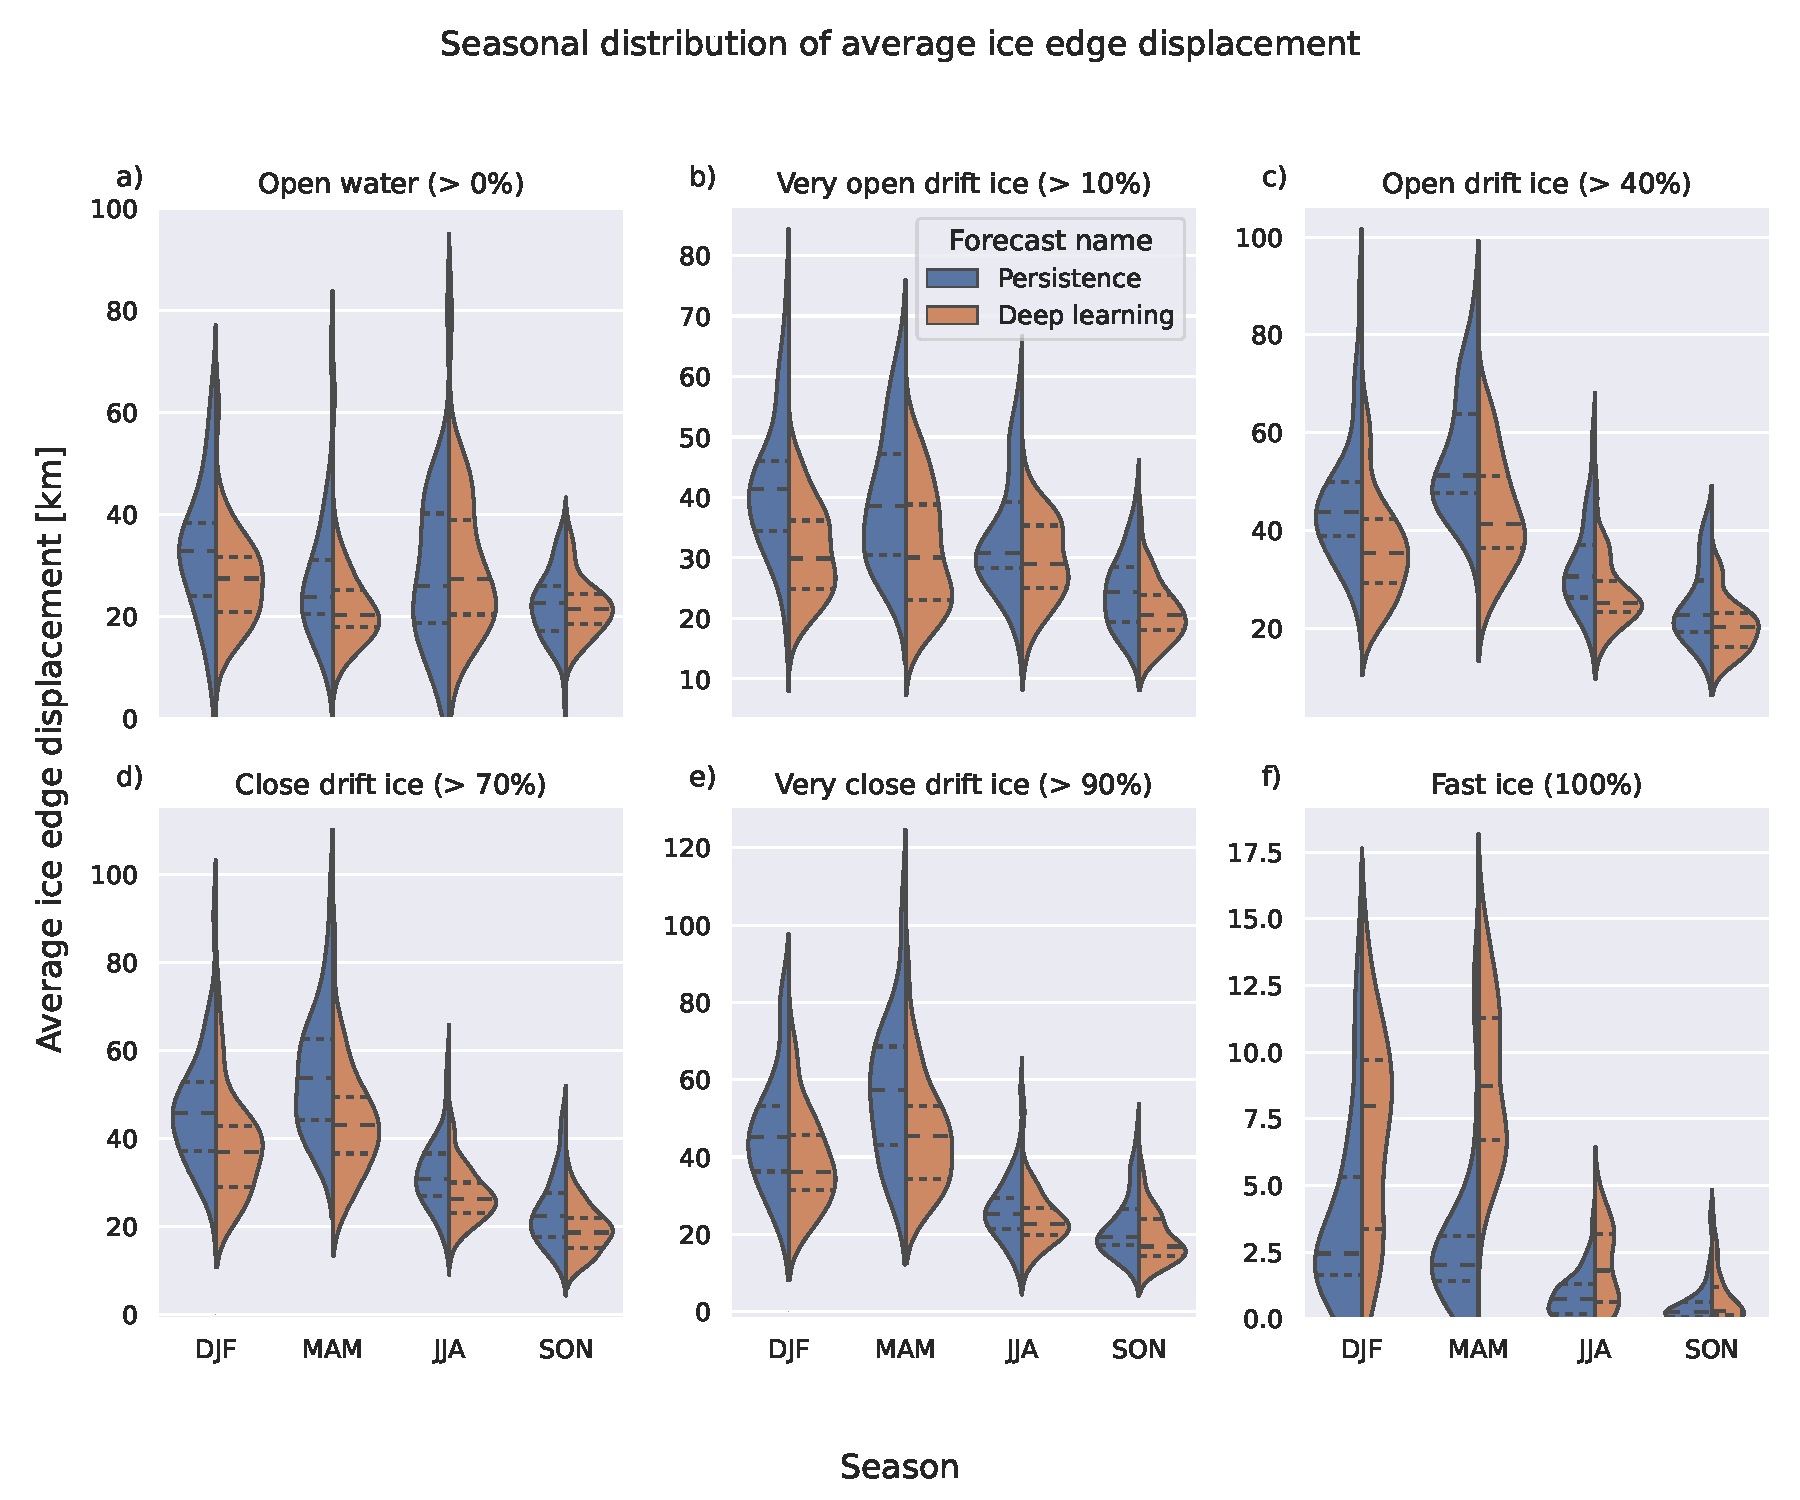
\includegraphics[width=\textwidth]{niiee}
    \caption{\label{fig:violins}Seasonal distribution of the mean ice edge displacement NIIEE for the different sea ice chart categories. The sea ice concentration range for each contour which denote the lower concentration threshold is also noted. The lower and upper dashed line denote the interquartile range, with the middlemost dashed line showing the distribution median.}
\end{figure}

Figures \ref{fig:mean_annual_confidence} and \ref{fig:confidence_seasonal} shows the deep learning model confidence as an annual mean for all output contours (Figure \ref{fig:mean_annual_confidence}) and the fast-ice contour distributed seasonally (Figure \ref{fig:confidence_seasonal}). The confidence values shown are output pixel values after the sigmoid (Equation \ref{eq:sigmoid}), such that values closer than 1 are pixels that the model is more confident to belong in the output contour. Likewise, values closer to 0 are confident not to belong to the targeted contour.

Figure \ref{fig:mean_annual_confidence} shows that all cumulative contours, except fast-ice, have a confidence pattern similar to the seasonal cycle of sea ice concentration. This is expected since for all contours and at all dates sea ice concentration is always present north of Svalbard and towards Greenland in the left of the model domain, whereas the less confident areas east of Svalbard exert spatial variability since the sea ice drifts and accumulates / melts. However, it is noted that the fast-ice contour (Figure \ref{fig:mean_annual_confidence}f) shows a lower overall confidence level, as well as only being restricted to the land structures present in the scene.

\begin{figure}
    \centering
    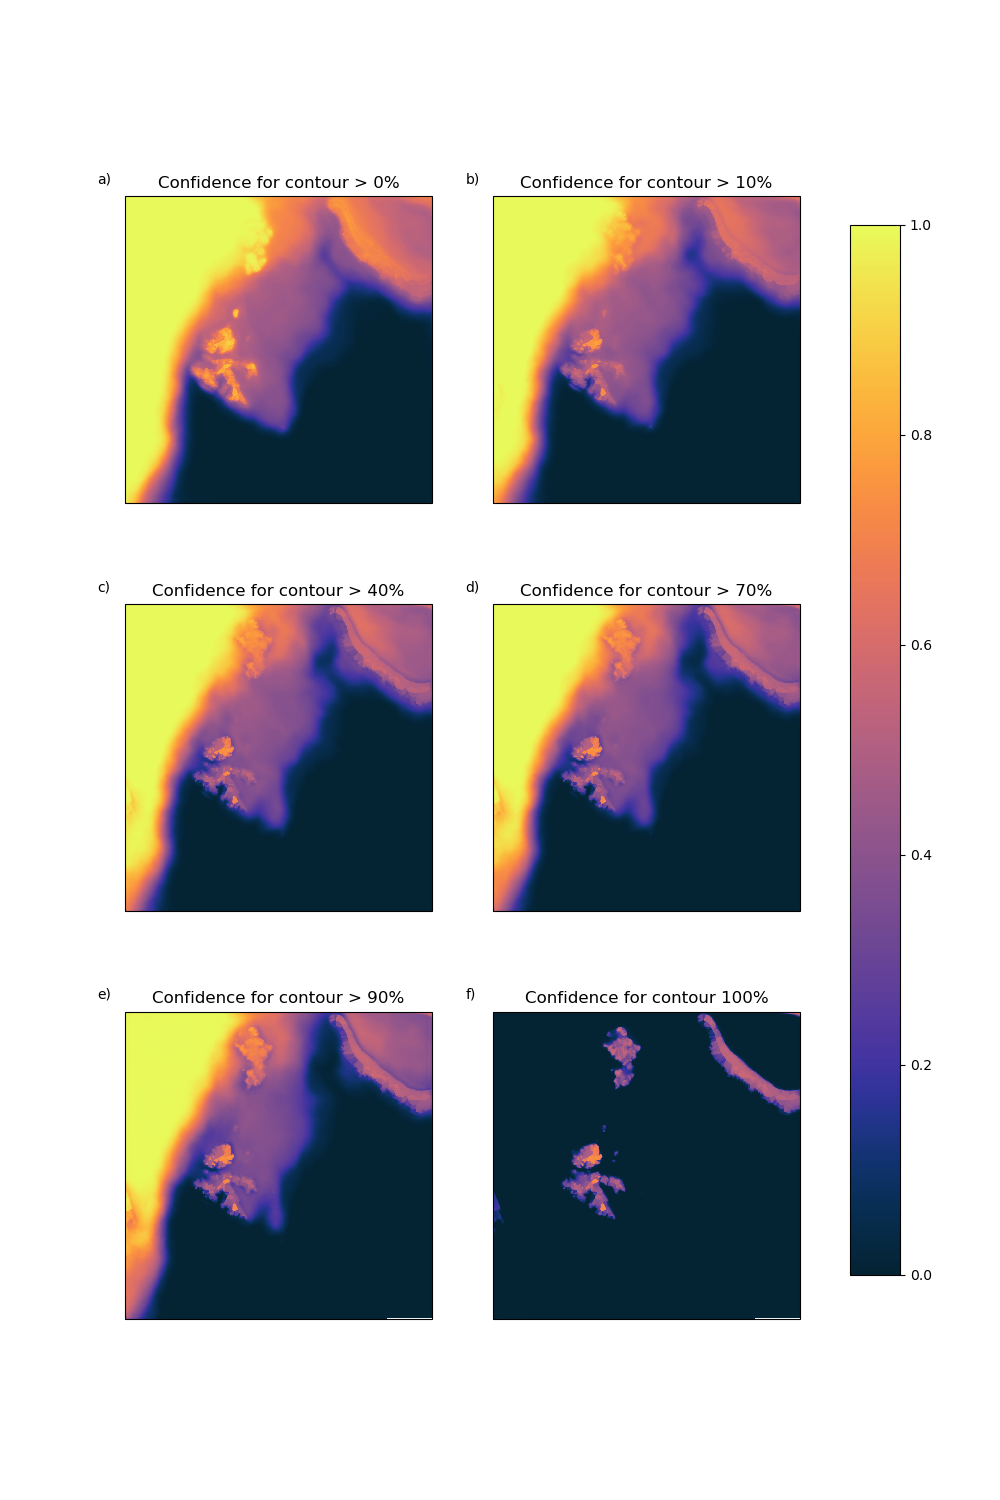
\includegraphics[width=.8\textwidth]{confidence_mean_annual}
    \caption{\label{fig:mean_annual_confidence}Mean annual probabilities for the different cumulative contours outputted by the deep learning model (the class ice free open water is not shown).}
\end{figure}

The seasonal confidence cycle for the fast-ice contour is shown in Figure \ref{fig:confidence_seasonal}. It is seen that the spatial distribution of confidence tends to resemble the land-covered pixels for all seasons, although with varying levels of confidence. E.g. Novaya Semlya is barely visible in Figure \ref{fig:confidence_seasonal}d.

\begin{figure}
    \centering
    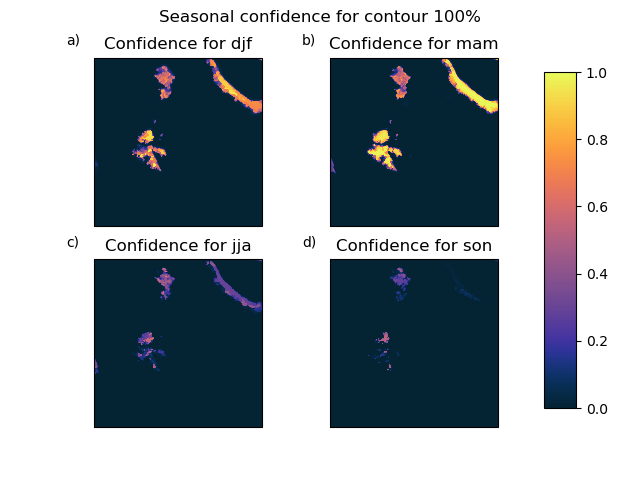
\includegraphics[width=\textwidth]{confidence_test_contour_6}
    \caption{\label{fig:confidence_seasonal}Mean seasonal confidence for the fast-ice cumulative contour.}
\end{figure}

The monthly mean sea ice edge length for the sea-ice charts and the predictions is shown in Figure \ref{fig:ice-edge-length}. The predicted ice edge follows a similar seasonal pattern to the ice edge length from the target ice charts. Each monthly mean predicted sea ice edge length is biased towards shorter lengths, and the bias increases with longer forecast lead-times.

\begin{figure}
    \centering
    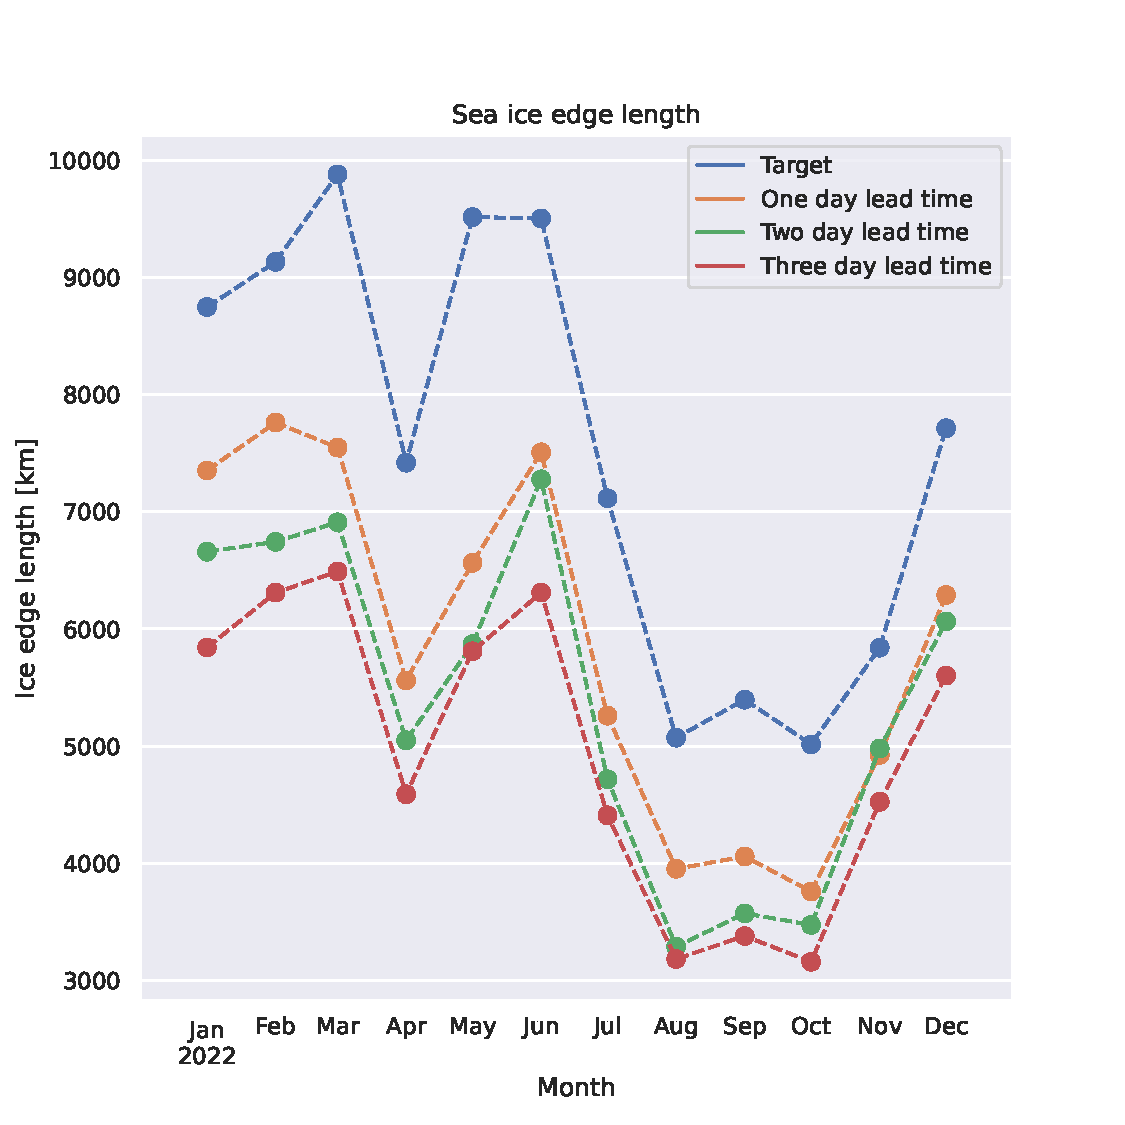
\includegraphics[width=\textwidth]{ice_edge_length}
    \caption{\label{fig:ice-edge-length}Mean monthly sea ice edge length for the entire 2022 test dataset. The ice edge is defined from a 10\% threshold, which results in the 10\% contour being used to define the ice edge. Each entry in the defined sea ice edge are on a 1km resolution. Each deep learning marker is annotated with the mean monthly bias with respect to the target sea ice edge length.}
\end{figure}

% Moreover, the monthly distribution of the different sea ice categories is shown in Figure \ref{fig:ice-contour-area}. The figure shows that the deep learning model resolve the area of each contour with a similar scale and variability as the target sea ice charts. 

% \begin{figure}
    % \centering
    % 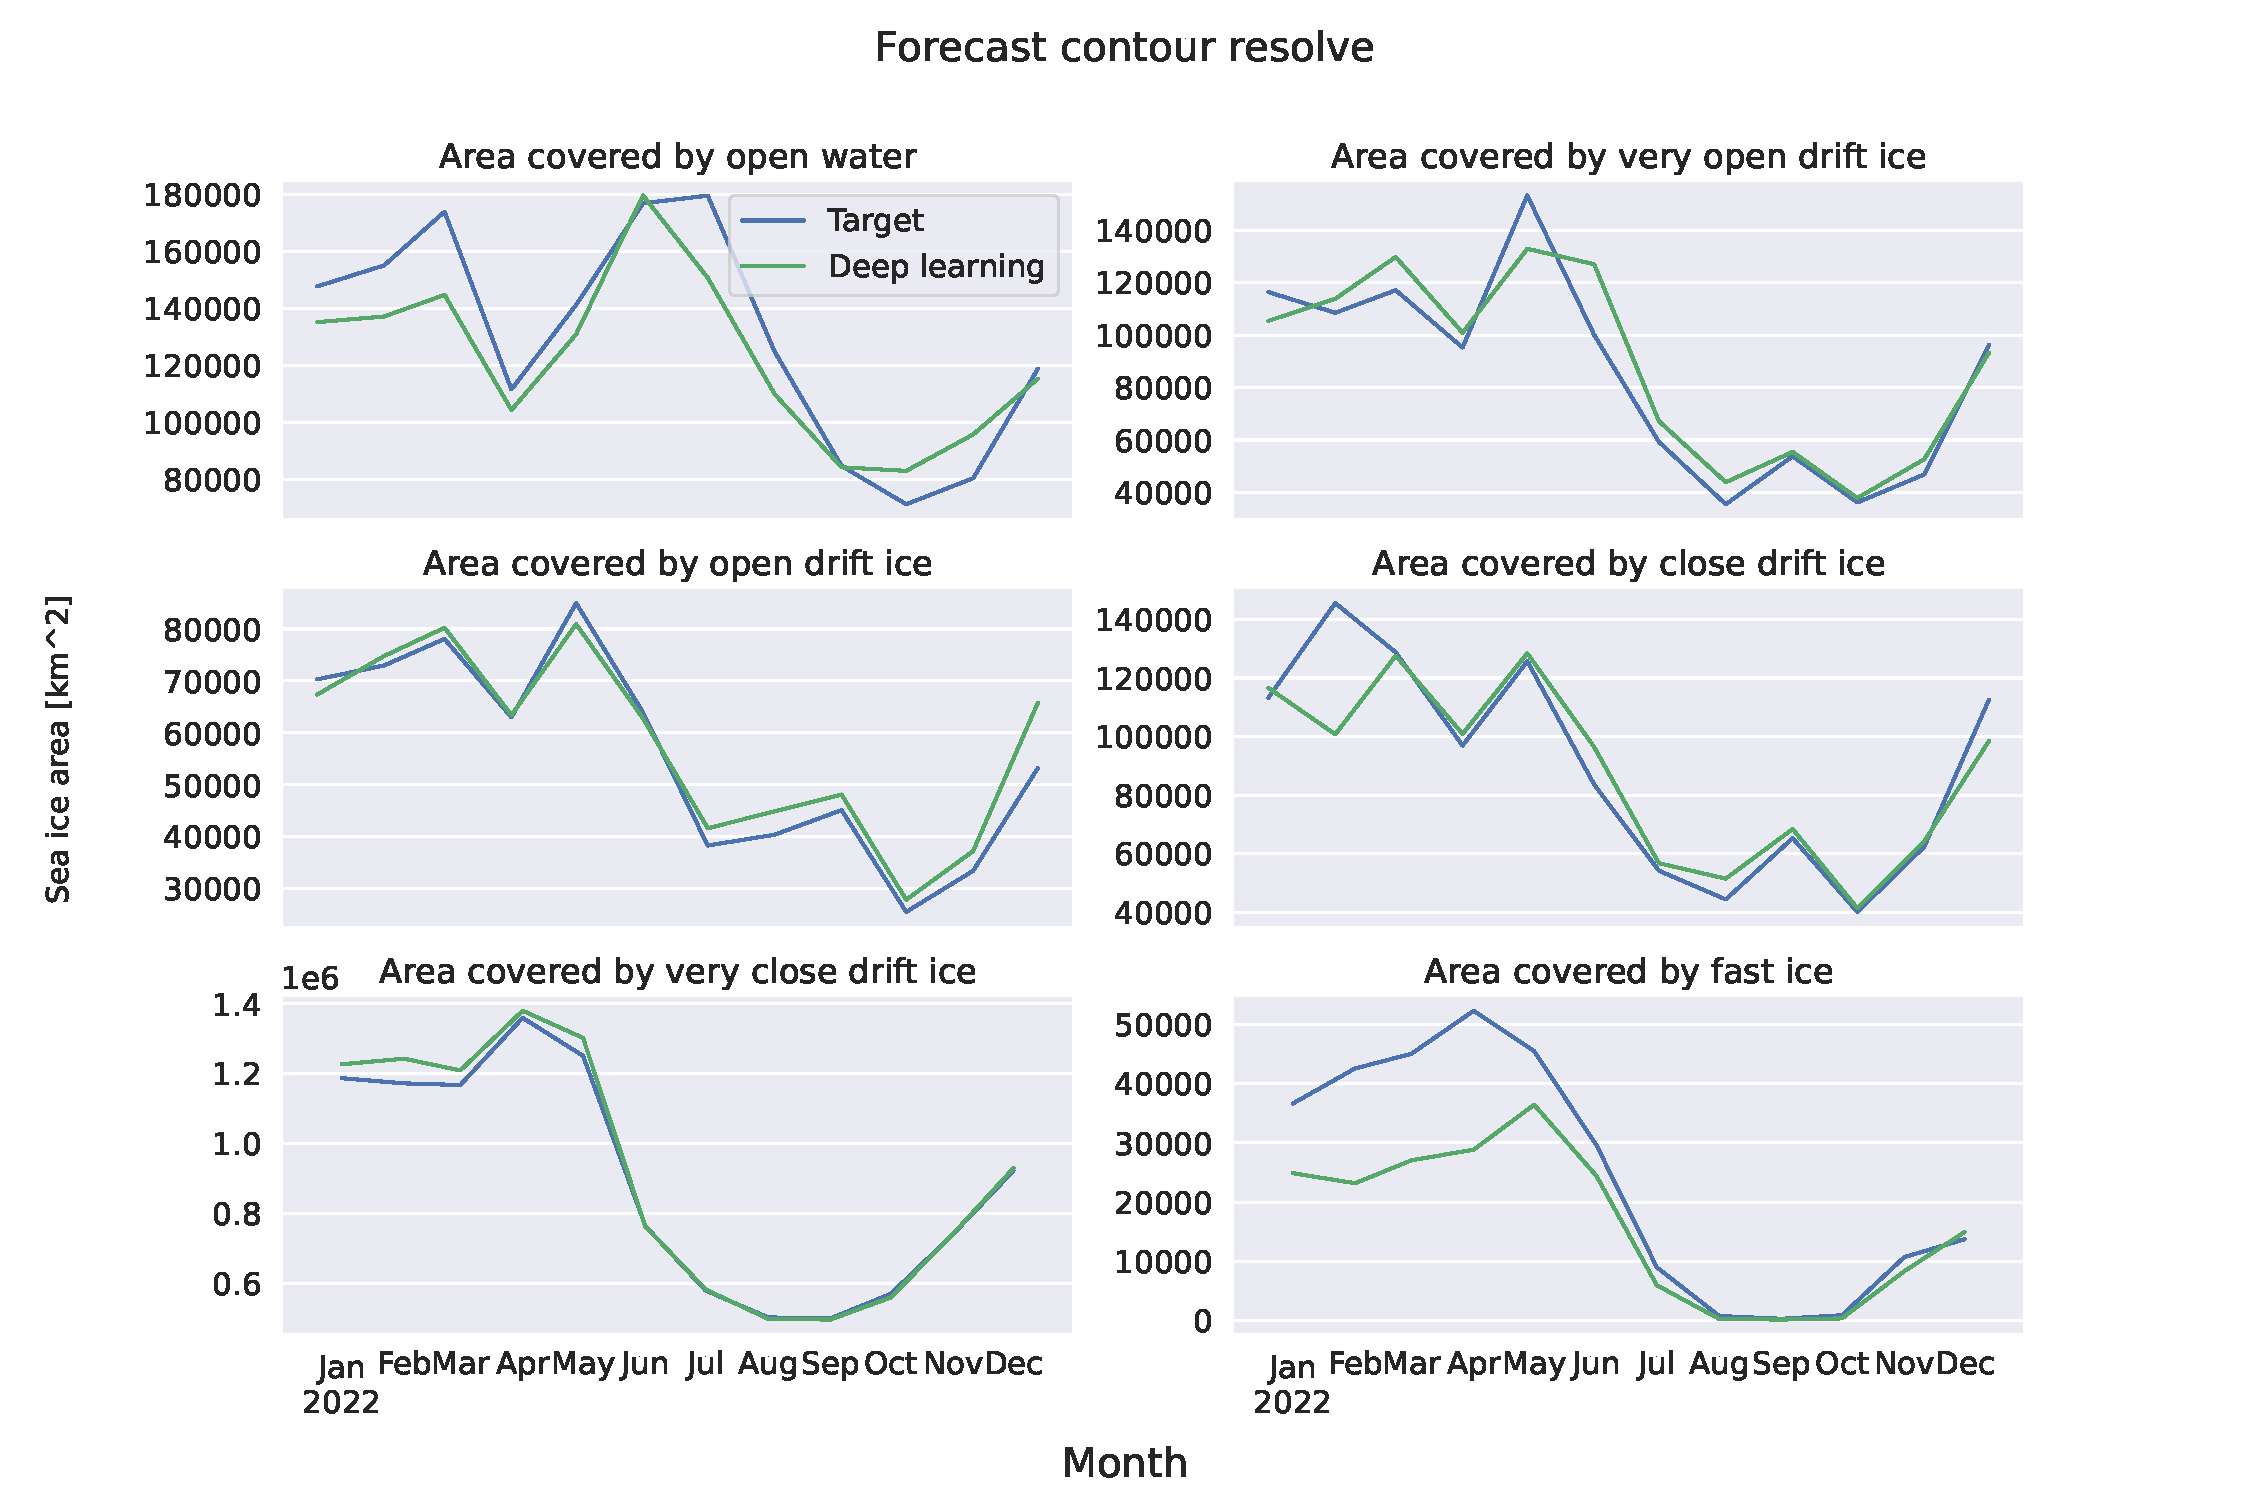
\includegraphics[width=\textwidth]{ice_contour_area}
    % \caption{\label{fig:ice-contour-area}Mean monthly sea ice category distribution for the model and the target sea ice charts for the 2022 test dataset. Each contour is represented by the sea ice area, which is computed from the sum of pixels in each contour times their spatial extent.}
% \end{figure}


\subsection{Intercomparison of sea-ice forecasts}
\label{sec:interproduct-compare}
This section covers results regarding the multi-product comparison. First, the preparation of samples as well as setup of the comparison environment is described. The physical models considered for this comparison are neXtSIM \citep{Williams2021} presented in Section \ref{sec:nextsim} and Barents-2.5 \citep{Roehrs2022} presented in Section \ref{sec:barents}, whereas the considered baseline-forecasts are persistence and the linear sea ice concentration trend described in Section \ref{sec:baselines}. Note for Barents-2.5 that only the ensemble member forced with atmospheric variables from AROME Arctic is utilized. Two different products are used as ground truth. The first product is the sea ice charts, which will be utilized similarly as when comparing only against persistence in Section \ref{sec:performance-persistence}. The second product to be utilized as ground truth is the independent AMSR2 observations produced by \citet{Spreen2008}.

When comparing against multiple products, the coarsest resolution model is used as a common spatial resolution. Also, the projection of the coarsest resolution is used for all products, such that other products have to be interpolated onto the grid of the coarsest resolution model, which is done using nearest neighbor interpolation. As both baselines-forecasts have a daily forecast frequency, comparing either with a deep learning prediction involves identifying the forecast with similar bulletin- and valid date, i.e. initialized at the same day and targeting the same lead time. When utilizing the sea ice charts as the ground truth, the spatial resolution of neXtSIM (3km) is the coarsest, and thus all products are interpolated onto the same resolution.

Comparing against the two physical models requires a consideration of the hourly forecast frequency \citep{Williams2021, Roehrs2022} of both models. First, given a published sea ice chart, the comparable physical model is initialized the following day at 00:00 UTC. Furthermore, a daily mean is computed from the 24 steps forward in time taken by the physical model when it covers the valid date of the deep learning forecast. Even though the sea ice charts only convey information about the sea ice concentration up until their publication time, the operational product is considered a reference for the entirety of the publication date. Moreover, to reduce introducing a bias towards the time of day to the physical forecasts as well as limiting the spatial variability induced by the lack of a temporal mean, reducing the physical forecasts to daily averages is considered a more comparable approach than e.g. selecting a single hour (15:00 UTC) from the forecasts.

Since the AMSR2 observations are supplied on a 6.25 km spatial resolution \citep{Spreen2008}, when AMSR2 is used as the ground truth all data is interpolated to match the resolution of AMSR2. Although the AMSR2 data have a substantially coarser spatial resolution compared to the sea ice charts or the deep learning system, the data makes it possible to assess the generalizability of the deep learning performance when targeting an unseen and independent ground truth.

From this setup, the mean of the first 24 hours of a forecast from a physical model is compared against a deep learning prediction with one day lead time, the mean between 24 and 48 hours are compared against a deep learning prediction with two day lead time and the mean of the third predicted day is compared against a deep learning prediction with three day lead time. Figure \ref{fig:product_compare_timeline} summarizes the process. Note that Barents-2.5 only has a 66 hour lead time \citep{Roehrs2022}, thus the mean between $t = 48$ and $t = 66$ is computed when comparing against a three day lead time prediction.

\begin{figure}
    \centering
    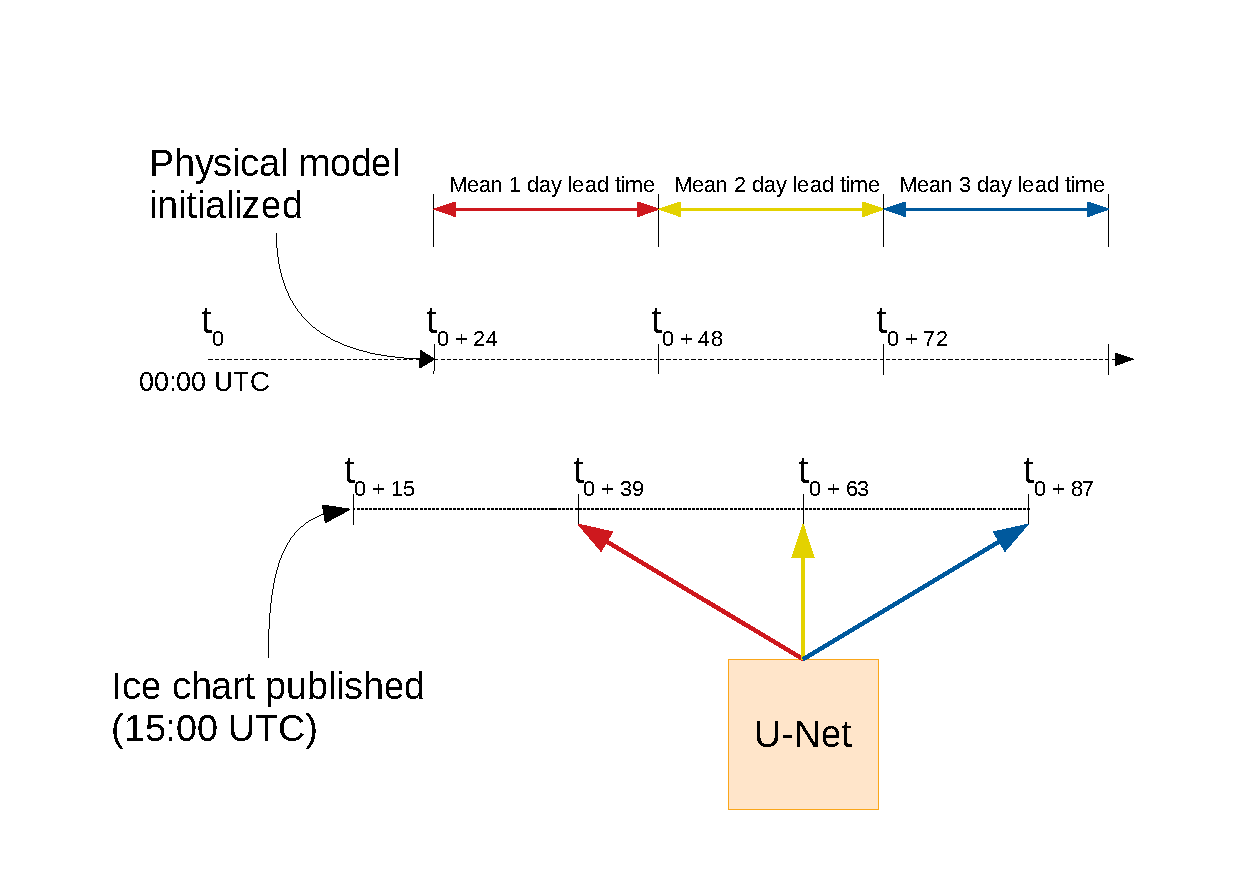
\includegraphics[width=\textwidth]{product_compare_timeline}
    \caption{\label{fig:product_compare_timeline}Overview describing how a physical model with an hourly frequency is compared against a deep learning forecast. Timestamps are hourly, and relative to 00:00 UTC the day a sea ice chart is published. The physical model is initialized the following day. Colors are used to denote lead time comparability, with red $= 1$, yellow $= 2$ and green $= 3$ day lead time.}
\end{figure}

It is noted that when comparing against multiple forecast products as described in Figure \ref{fig:product_compare_timeline}, only the common dates shared between all products are used. With the current setup, where neXtSIM, Persistence, deep learning, OSI SAF trend and Barents-2.5 are considered, the test dataset is reduced from 196 to 171 samples, 147 to 130 samples and 142 to 125 samples for 1, 2, and 3 day lead time respectively. Moreover, Barents-2.5 is only considered starting with the month of June, to comply with the spin up time of its data assimilation system \citep{Roehrs2022}.

Figure \ref{fig:model_compare} shows the seasonal distribution of NIIEE for the different forecast systems and benchmarks, following the setup described in Figure \ref{fig:product_compare_timeline}. By inspecting Figure \ref{fig:model_compare}, it can be seen that only the products based on the sea ice chart are able to achieve consistently low NIIEE for the $<10\%$ contour. Furthermore, for the (10 - 30\%, 40 - 60\%, 70 - 80\%, 90 - 100\%) contours, the deep learning system achieves the lowest median and mean values compared to all the other products. It can also be seen that neXtSIM tends to increase its mean and median as well as spread for increasing contours, with a similar although not as consistent pattern for Barents-2.5. Moreover, the OSI SAF trend typically has the highest valued outliers in the displayed ranges. Finally, no product is able to achieve a lower mean or median NIIEE compared to persistence when inspecting the (fast ice) contour. 

\begin{figure}
    \centering
    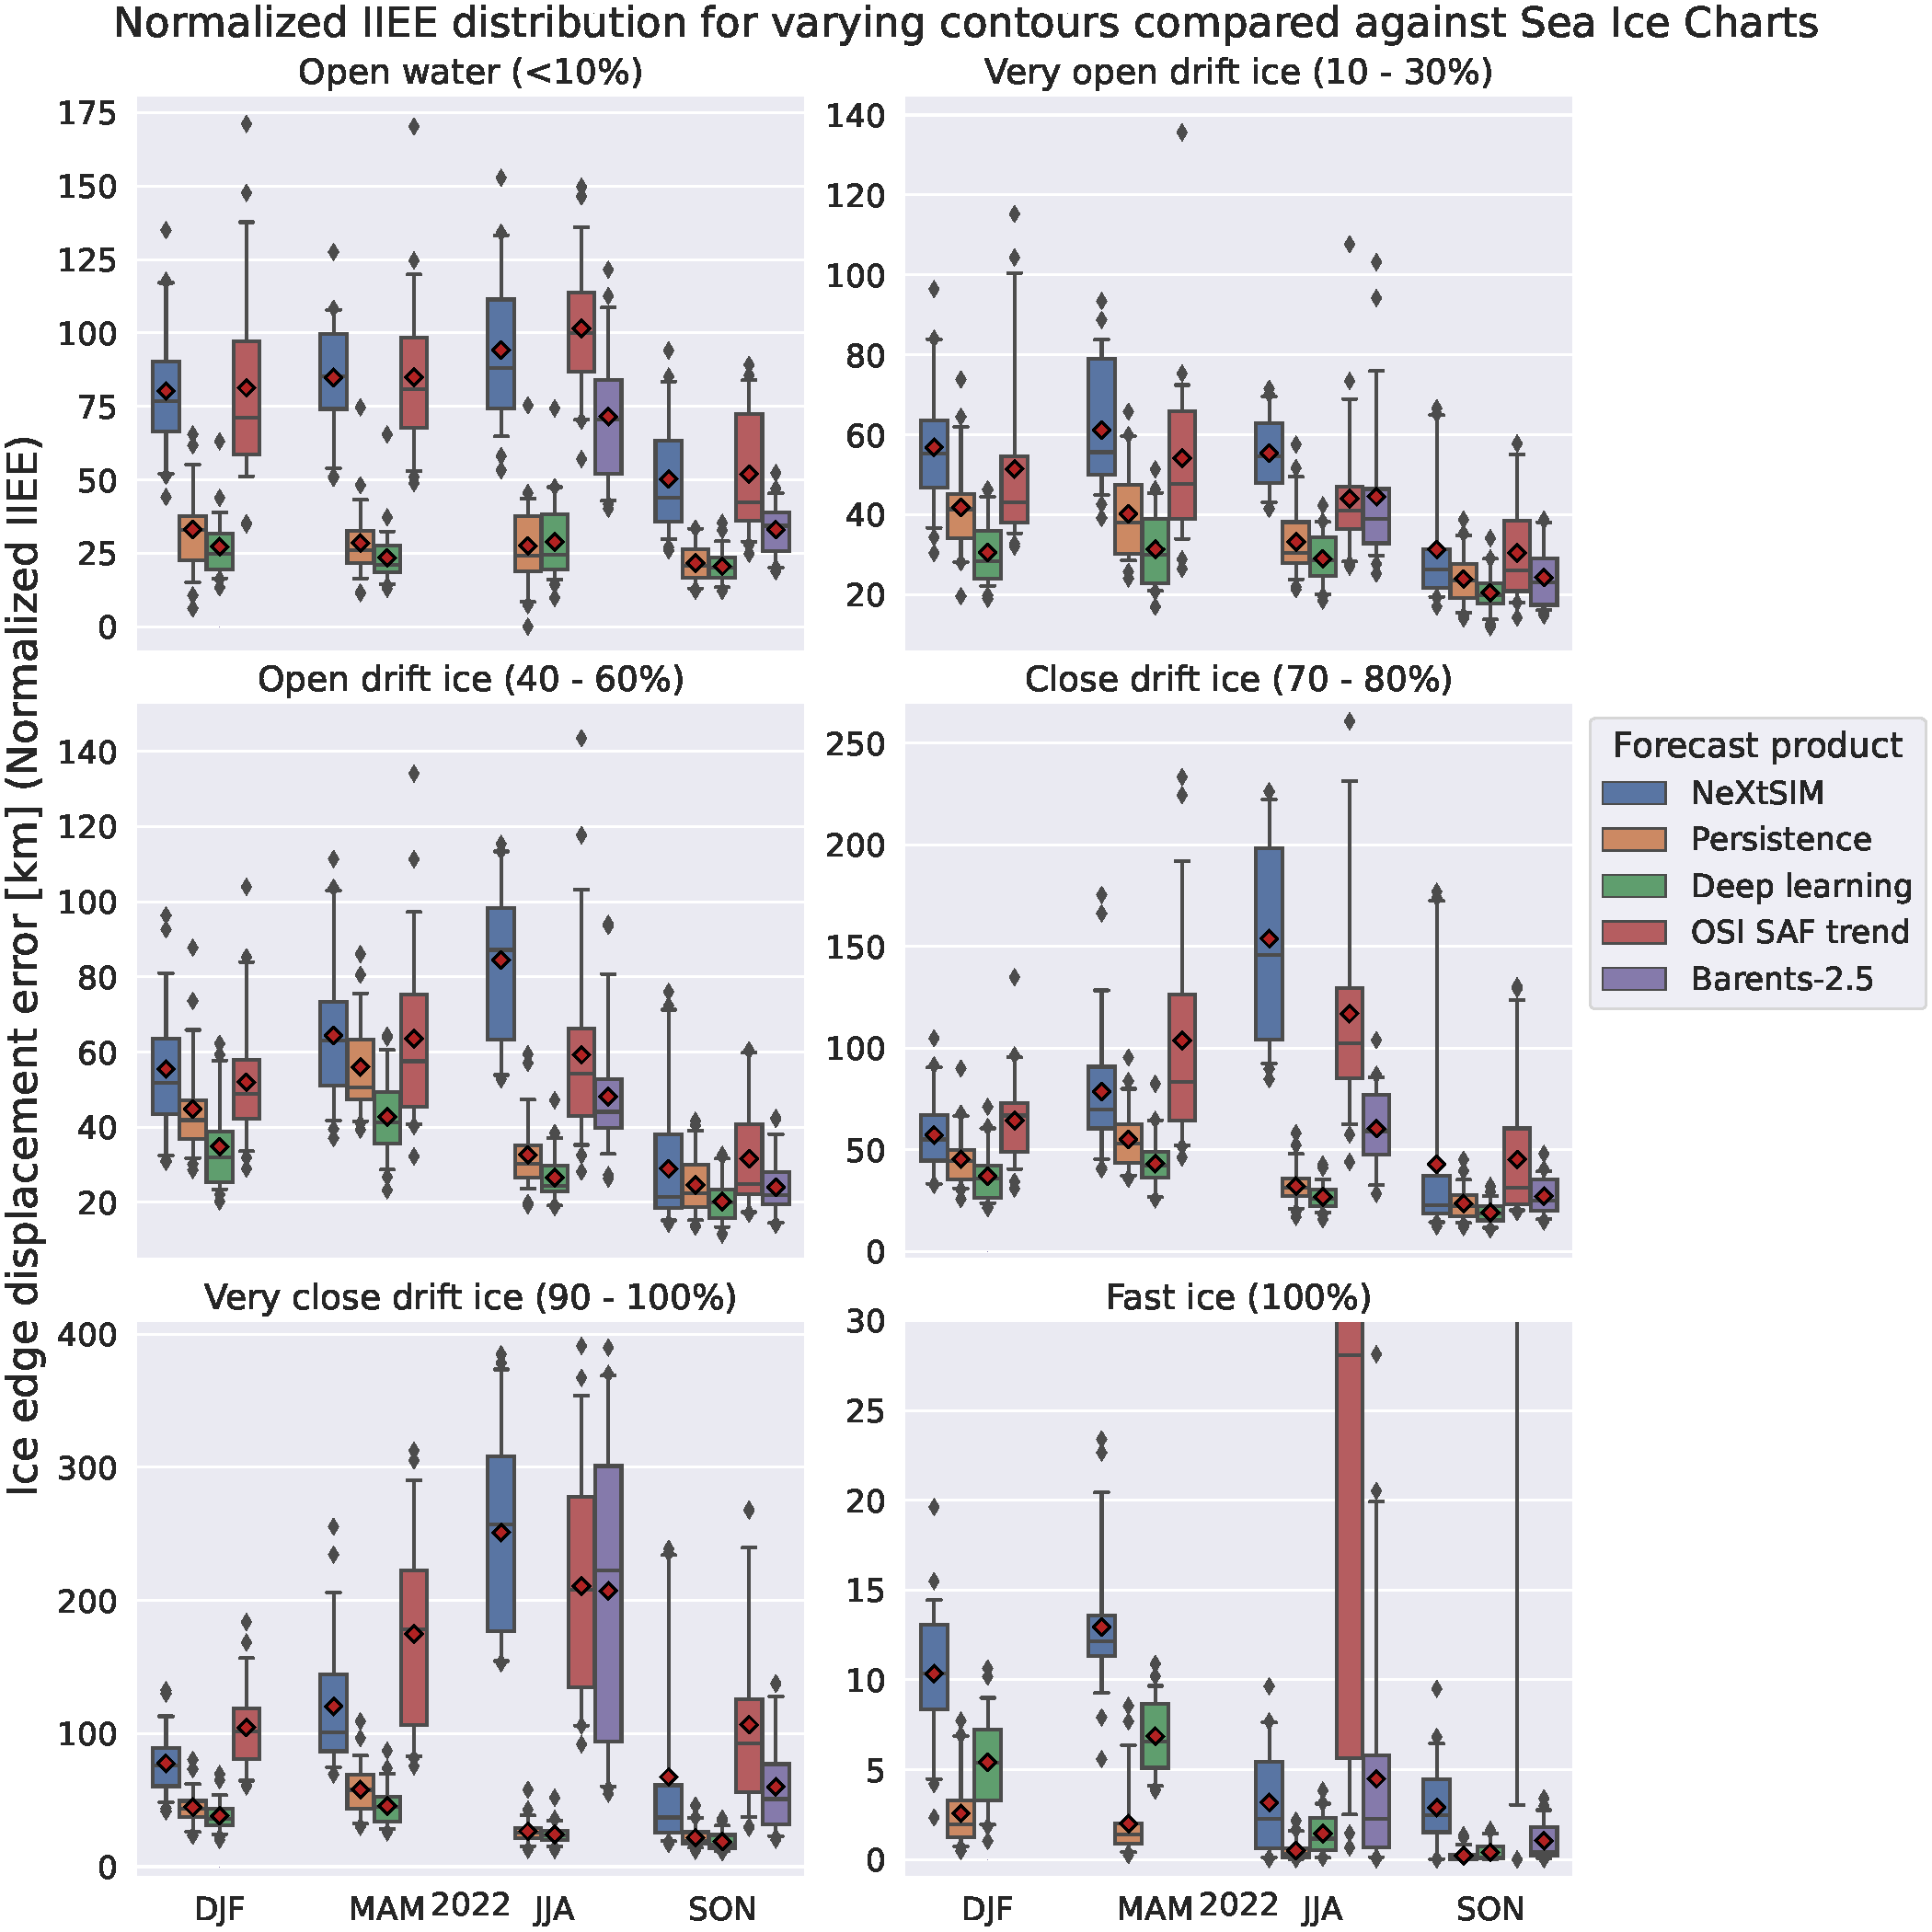
\includegraphics[width=\textwidth]{model_intercomparisson.pdf}
    \caption{\label{fig:model_compare}Model intercomparisson with a two day lead time. The boxes are constructed from seasonally distributed NIIEE values computed from the test dataset (2022). The sea ice charts are considered as targets. Each box cover the interquartile range (25th - 75th percentile), with whiskers covering the 5th and 95th percentile. The line in each box is the median, and the red diamond is the mean. The IIEE is normalized according to the climatological sea ice edge at the forecast valid date. The extent of the y axis is limited in such a way that the distributions are easily readable, at the expense of some outliers not being visible. The OSI SAF trend is computed from the past 7 days.}
\end{figure}

The fraction of days where the deep learning system achieves lower NIIEE compared to each considered product is shown in Figure \ref{fig:days-beat}. The deep learning system consistently achieves a $\geq50\%$ success rate compared to all products, except for persistence-forecast with 1 day lead time in July, August and September as well as Barents-2.5 2 day lead time in November and December. When compared to neXtSIM at 1 day lead time (Figure \ref{fig:days-beat}a), the deep learning system achieves a lower NIIEE at all considered dates in the test data. However, it can also be seen that a lower amount of days with lower NIIEE than neXtSIM are achieved as the lead time increases. The same pattern may also be seen in the Barents-2.5 data as the mean fraction of days with lower NIIEE for the deep learning system also decrease with lead time, although Barents-2.5 is only able to achieve lower NIIEE more than 50\% of the dates for a 2 day lead time as previously noted. With respect to persistence, the deep learning forecasts seem to achieve a higher fraction of days with lower NIIEE as lead time increases, although there is no trend for the individual months. At the (10 - 30\%) contour, the OSI SAF trend is consistently beat by the deep learning system during Winter and Spring, with less consistency observed during the Summer and Autumn seasons.

\begin{figure}
    \centering
    \begin{subfigure}{0.32\textwidth}
        \caption{1 day lead time}
        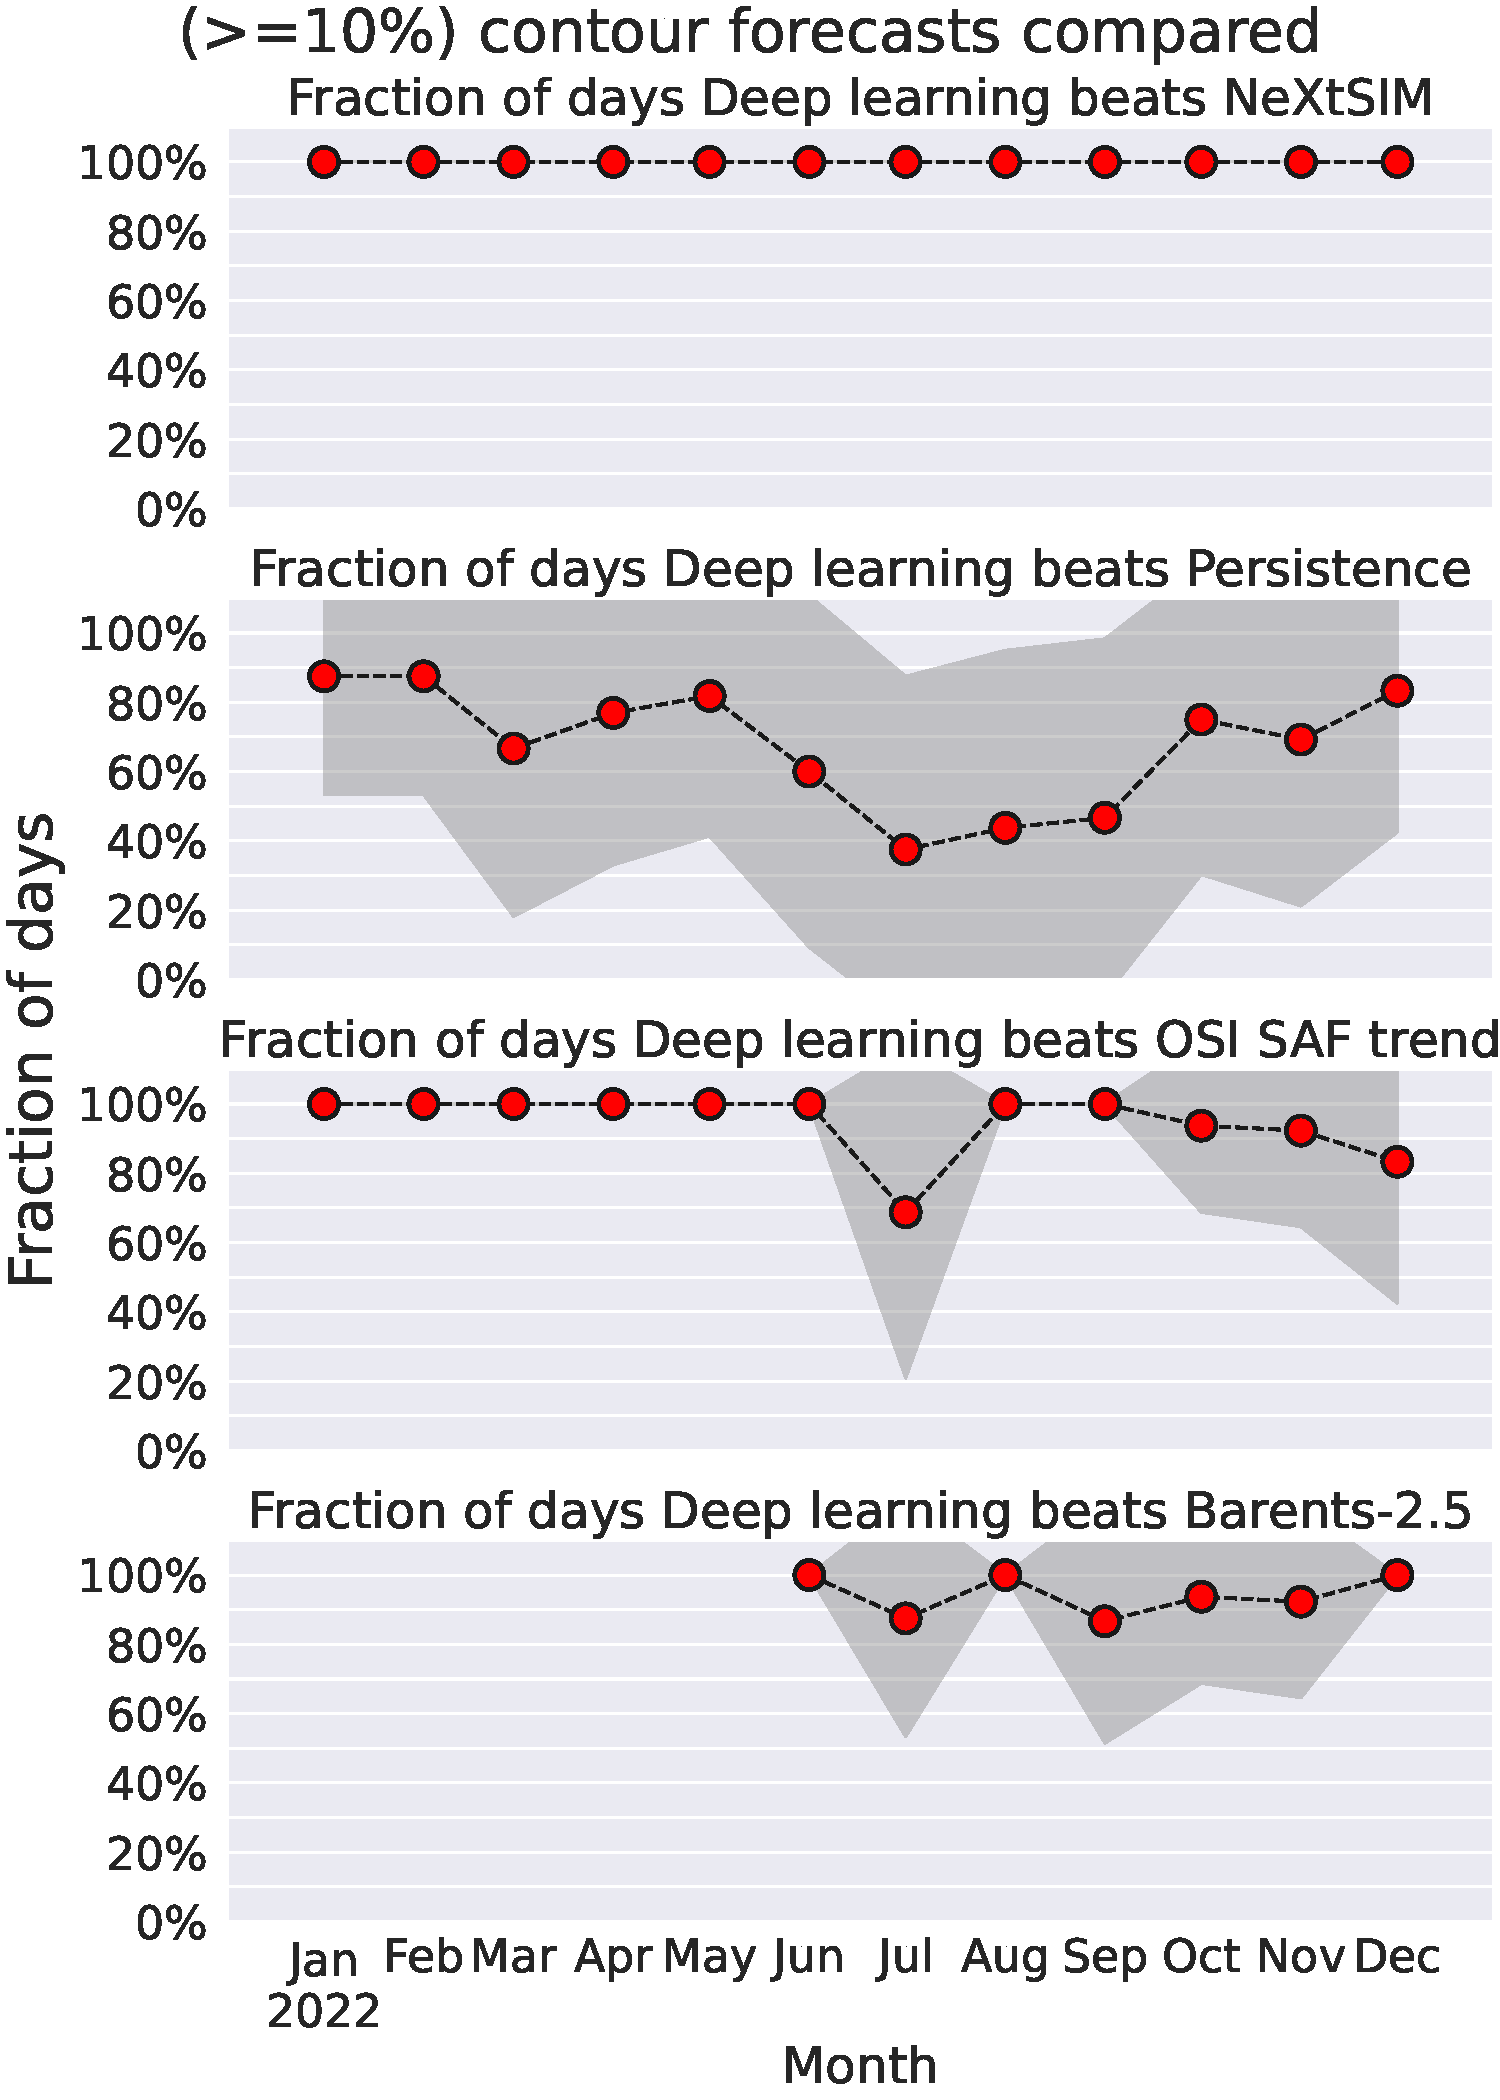
\includegraphics[width=\textwidth]{days_beat_weights_08031256.pdf}
    \end{subfigure}
    \begin{subfigure}{0.32\textwidth}
        \caption{2 day lead time}
        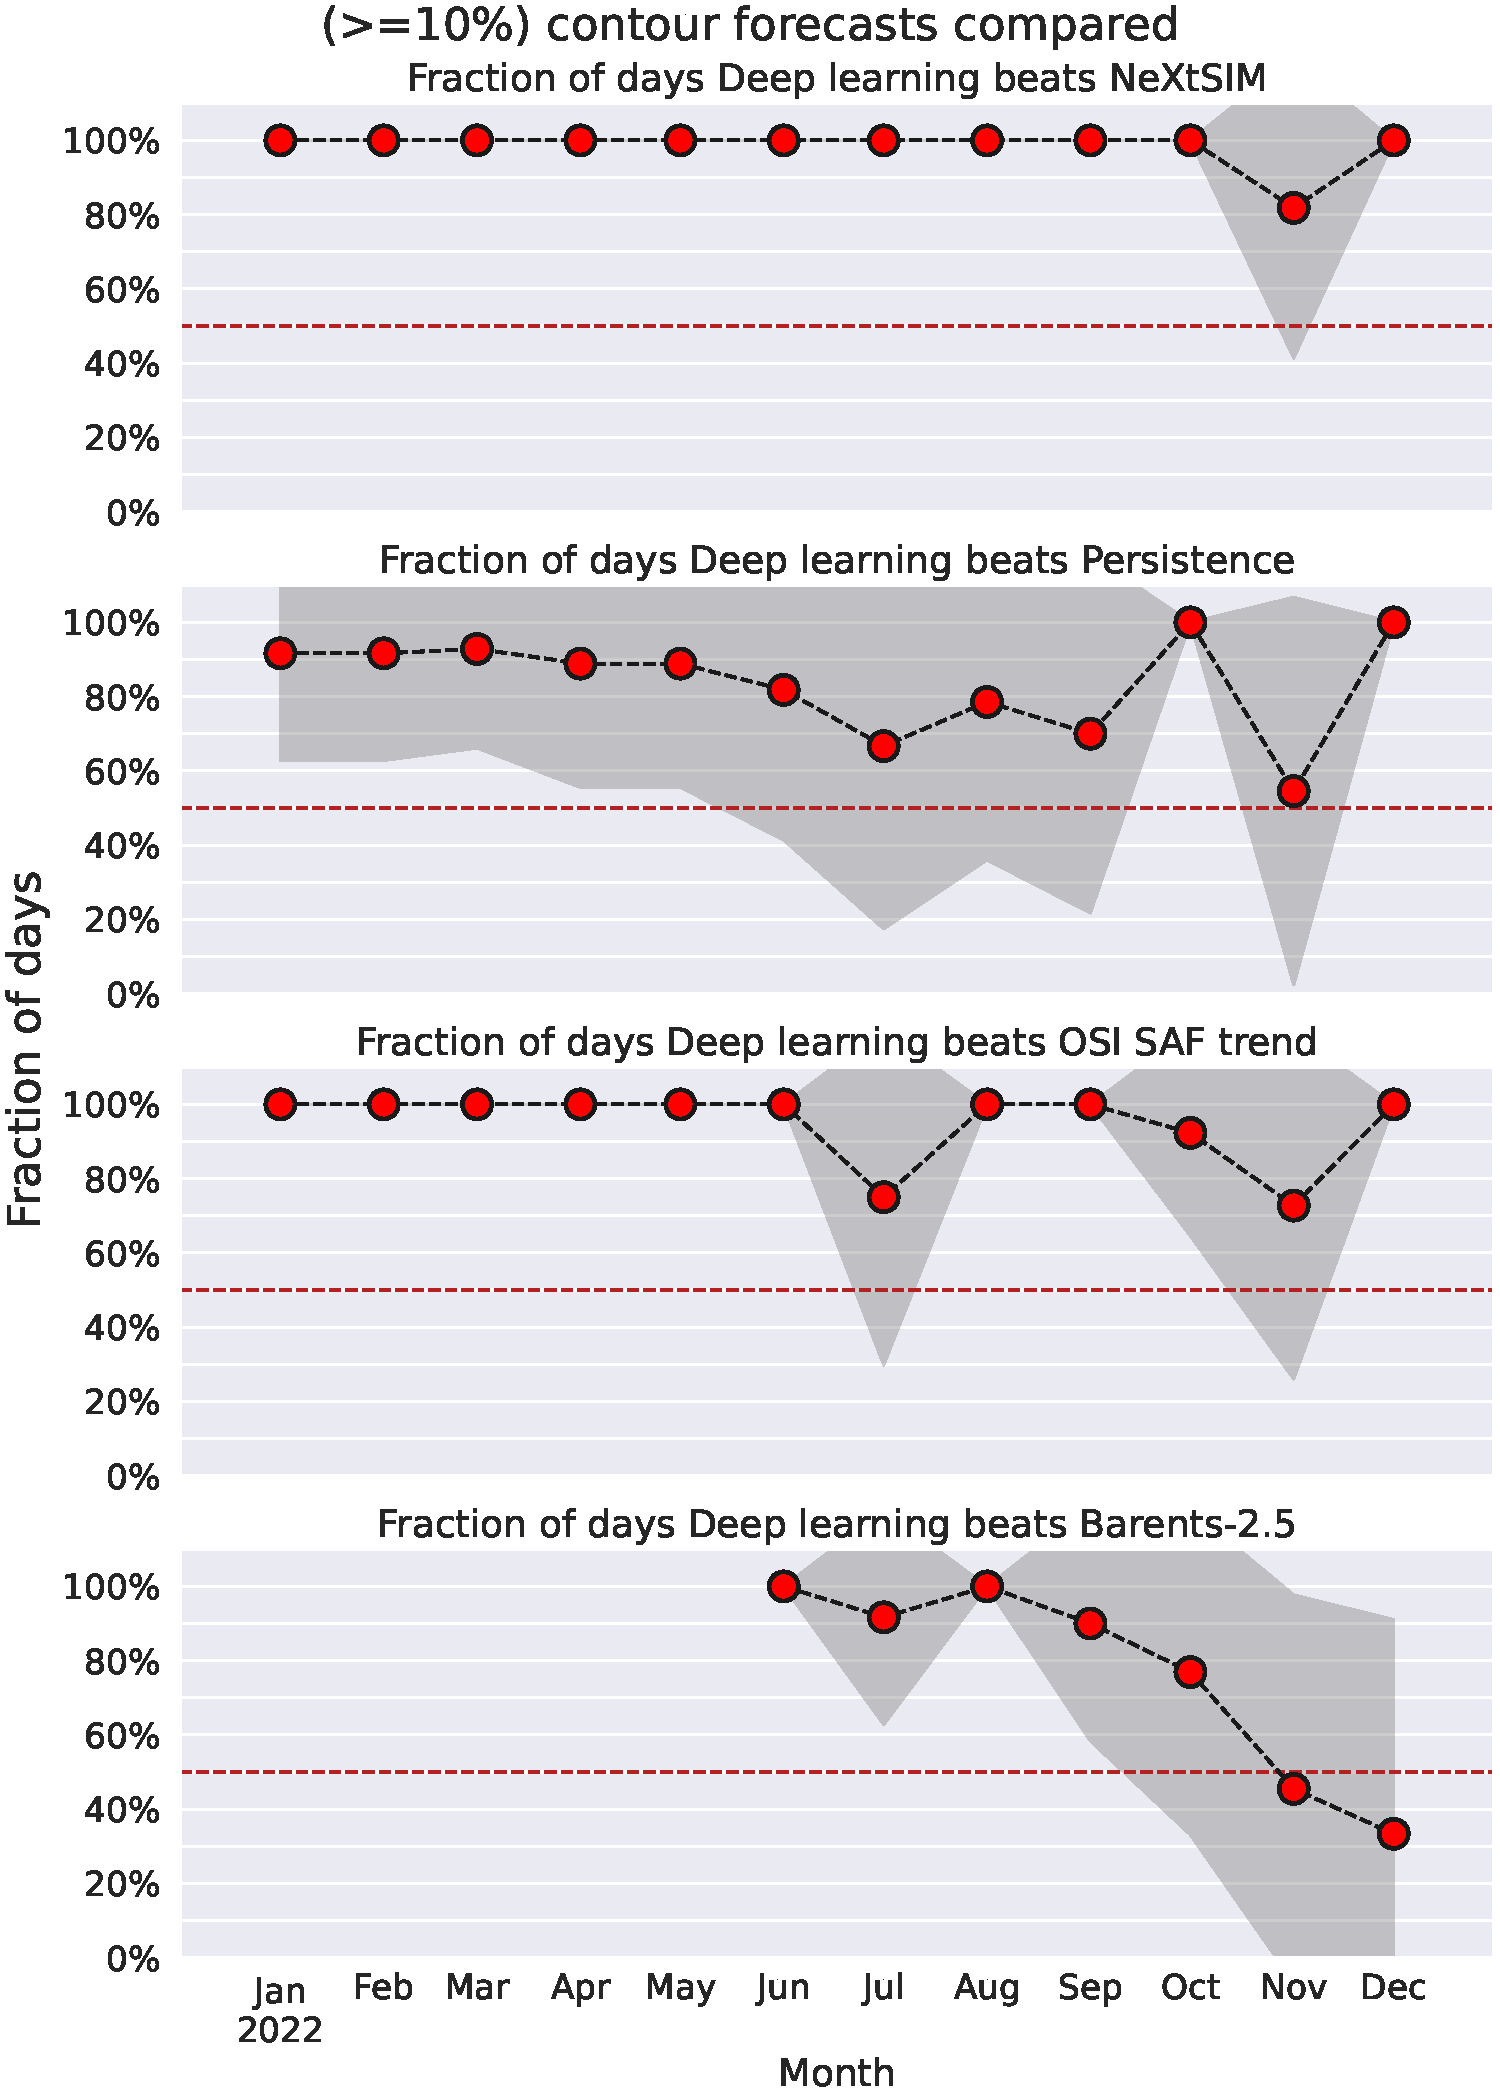
\includegraphics[width=\textwidth]{days_beat_weights_21021550.pdf}
    \end{subfigure}
    \begin{subfigure}{0.32\textwidth}
        \caption{3 day lead time}
        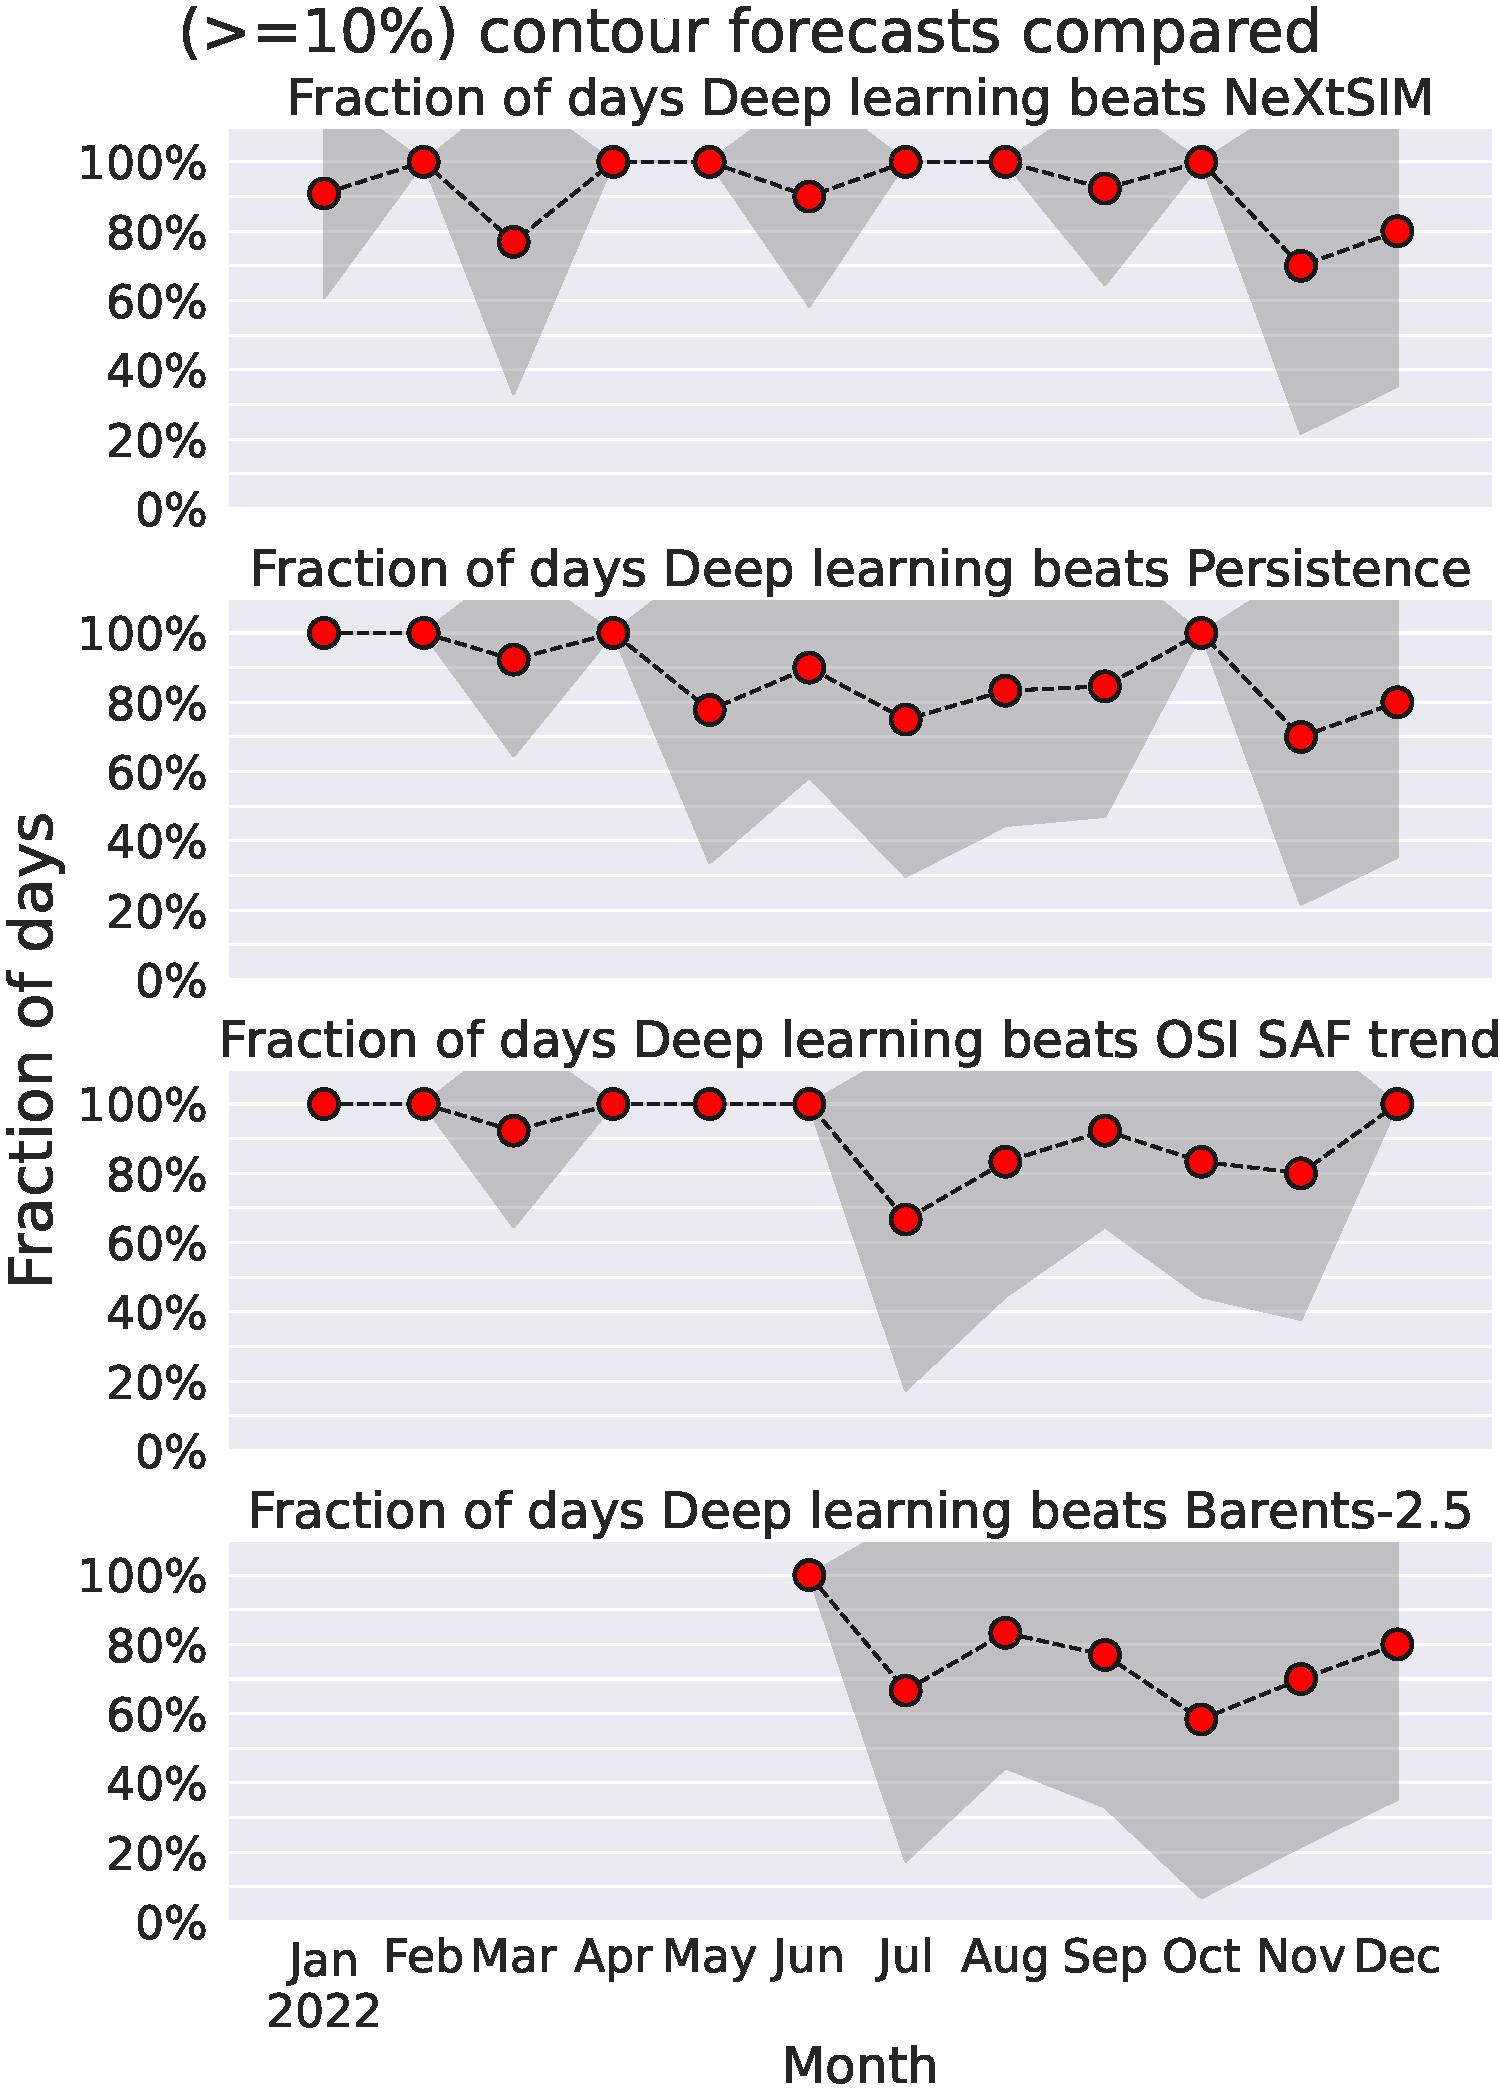
\includegraphics[width=\textwidth]{days_beat_weights_09031047.pdf}
    \end{subfigure}
    \caption{\label{fig:days-beat}Fraction of days where the deep learning forecast achieves a lower NIIEE than the compared product, distributed monthly for all lead times. Only the (10 - 30\%) contour has been considered, due to the relevance of the contour with respect to the definition of the sea ice edge and its application to operational end users. The red dashed line denotes the 50\% line. Gray contours denote the uncertainty (standard deviation) for each month. The sea ice chart has been used as ground truth target when computing the IIEE, and the score has been normalized according to the climatological sea ice edge.}
\end{figure}

The spatial distribution of product error is shown in Figure \ref{fig:anomalies}. It can be seen that both products which are based on the sea ice charts (deep learning system and persistence-forecasts) have lower bias than the three other products, as well as only exerting biases in the MIZ. Moreover, it can be seen from the top row in Figure \ref{fig:anomalies} the neXtSIM data have a negative bias along the sea ice edge, which is prominent during Winter and Spring. Moreover, the OSI SAF trend seem to have a strong negative bias along a wide sea ice edge. Finally, Barents-2.5 seem to have a positive bias around Svalbard in the Summer, with a less prominent overall bias during the Fall.

\begin{figure}
    \centering
    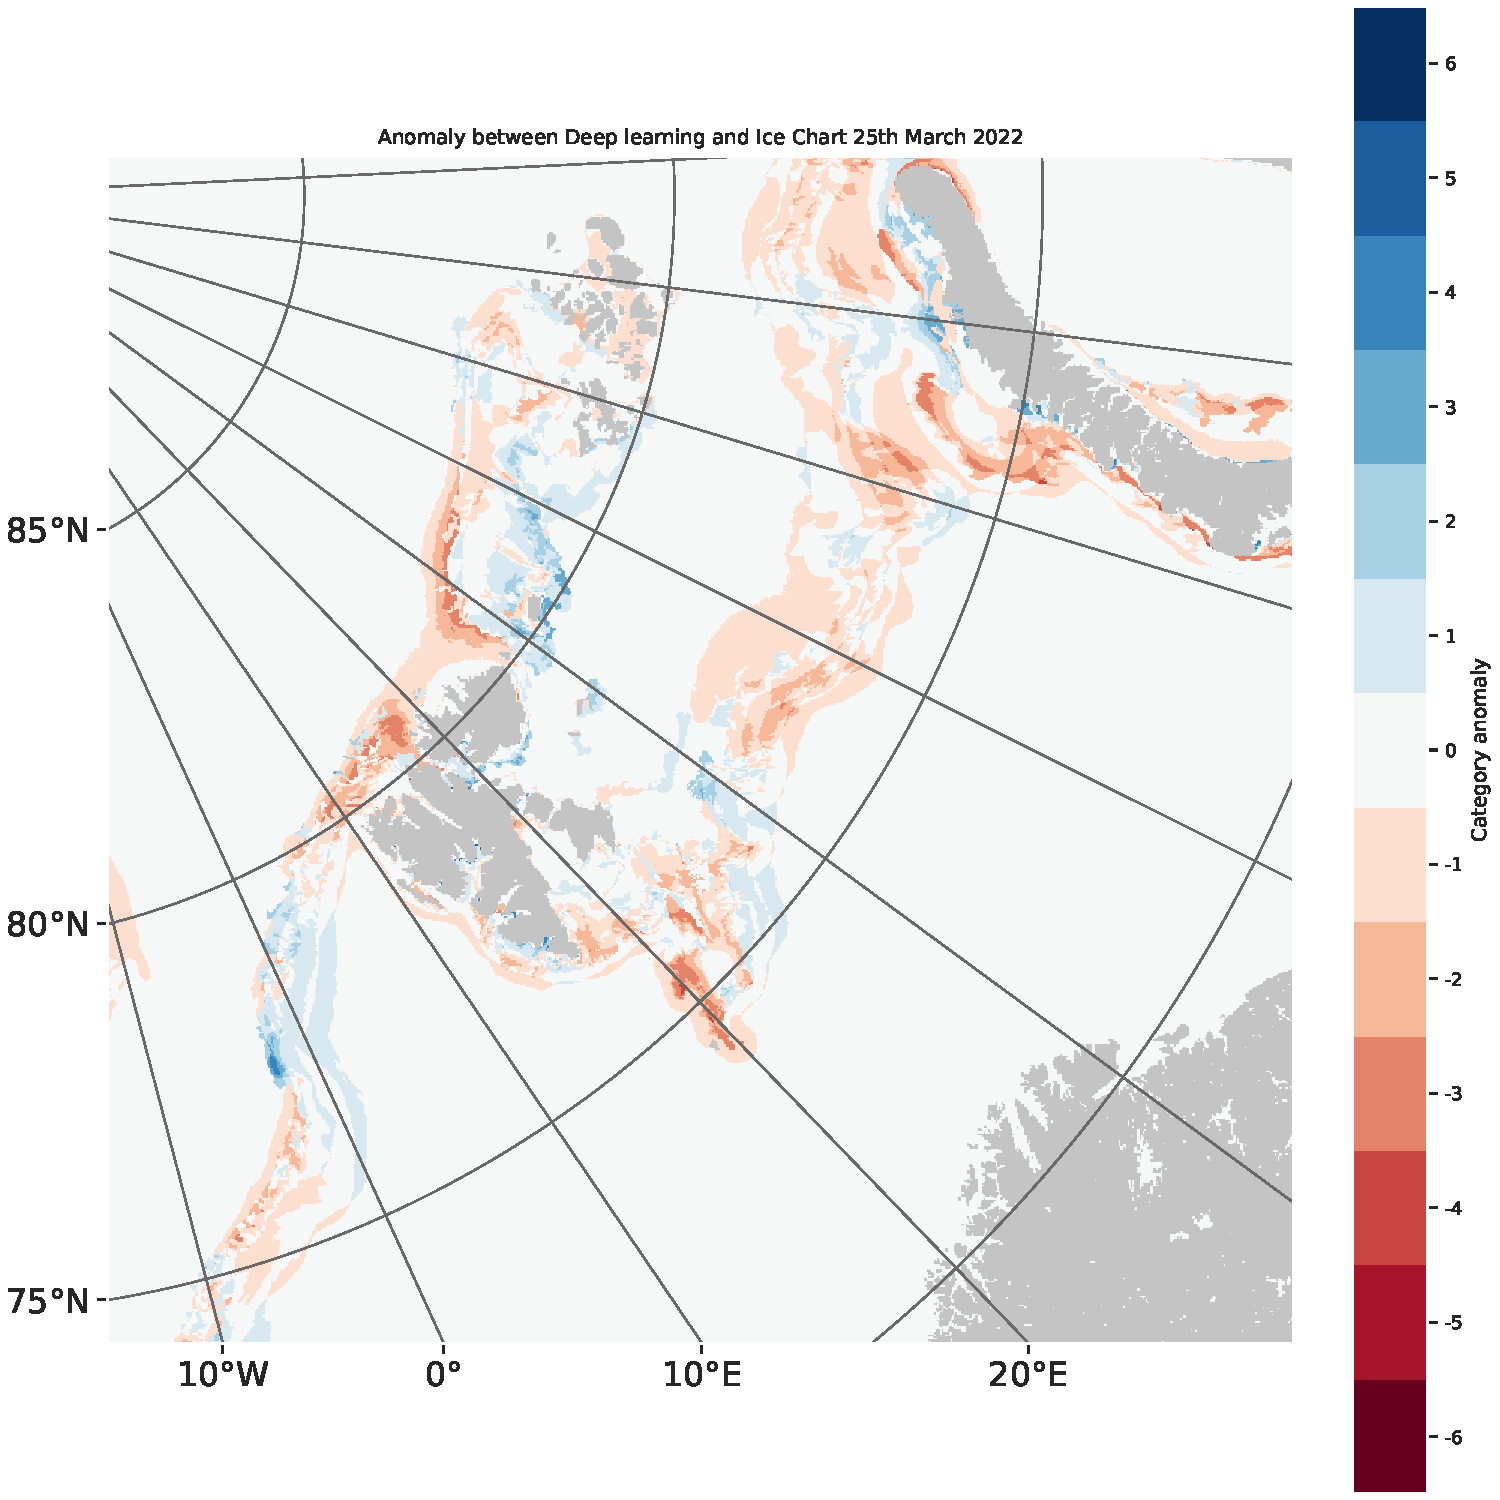
\includegraphics[width=\textwidth]{anomalies}
    \caption{\label{fig:anomalies}Spatial distribution of the mean seasonal error for predicted sea ice categories between the compared products. The data is interpolated onto the neXtSIM grid, and the test dataset is considered.}
\end{figure}


The seasonal NIIEE distributions shown in Figure \ref{fig:model_compare_amsr2} is created similarly as Figure \ref{fig:model_compare}, but with AMSR2 as the ground truth data, which also implies that all data have been interpolated onto the 6.25km AMSR2 grid \citep{Spreen2008}. Contrary to what was observed in Figure \ref{fig:model_compare}, the both the deep learning system and persistence-forecasts in Figure \ref{fig:model_compare_amsr2} exert significantly higher NIIEE at the <10\% contour. However, Barents-2.5 also exert a similar increased NIIEE as the deep learning system and persistence-forecasts at the same contour. Moreover, both the deep learning system and persistence-forecasts are within the interquartile range of neXtSIM and OSI SAF trend starting at the (10 - 30\%) contour. At the <10\% and (10 - 30\%) contours, the OSI SAF trend exerts the lowest mean and median NIIEE for all months except SON where neXtSIM achieves the lowest median and mean. However, starting at the (40 - 60\%) contour the deep learning system has the lowest median and mean NIIEE, which lasts until the fast-ice contour where performance is comparable between all products except for the OSI SAF trend during Winter and Spring.

\begin{figure}
    \centering
    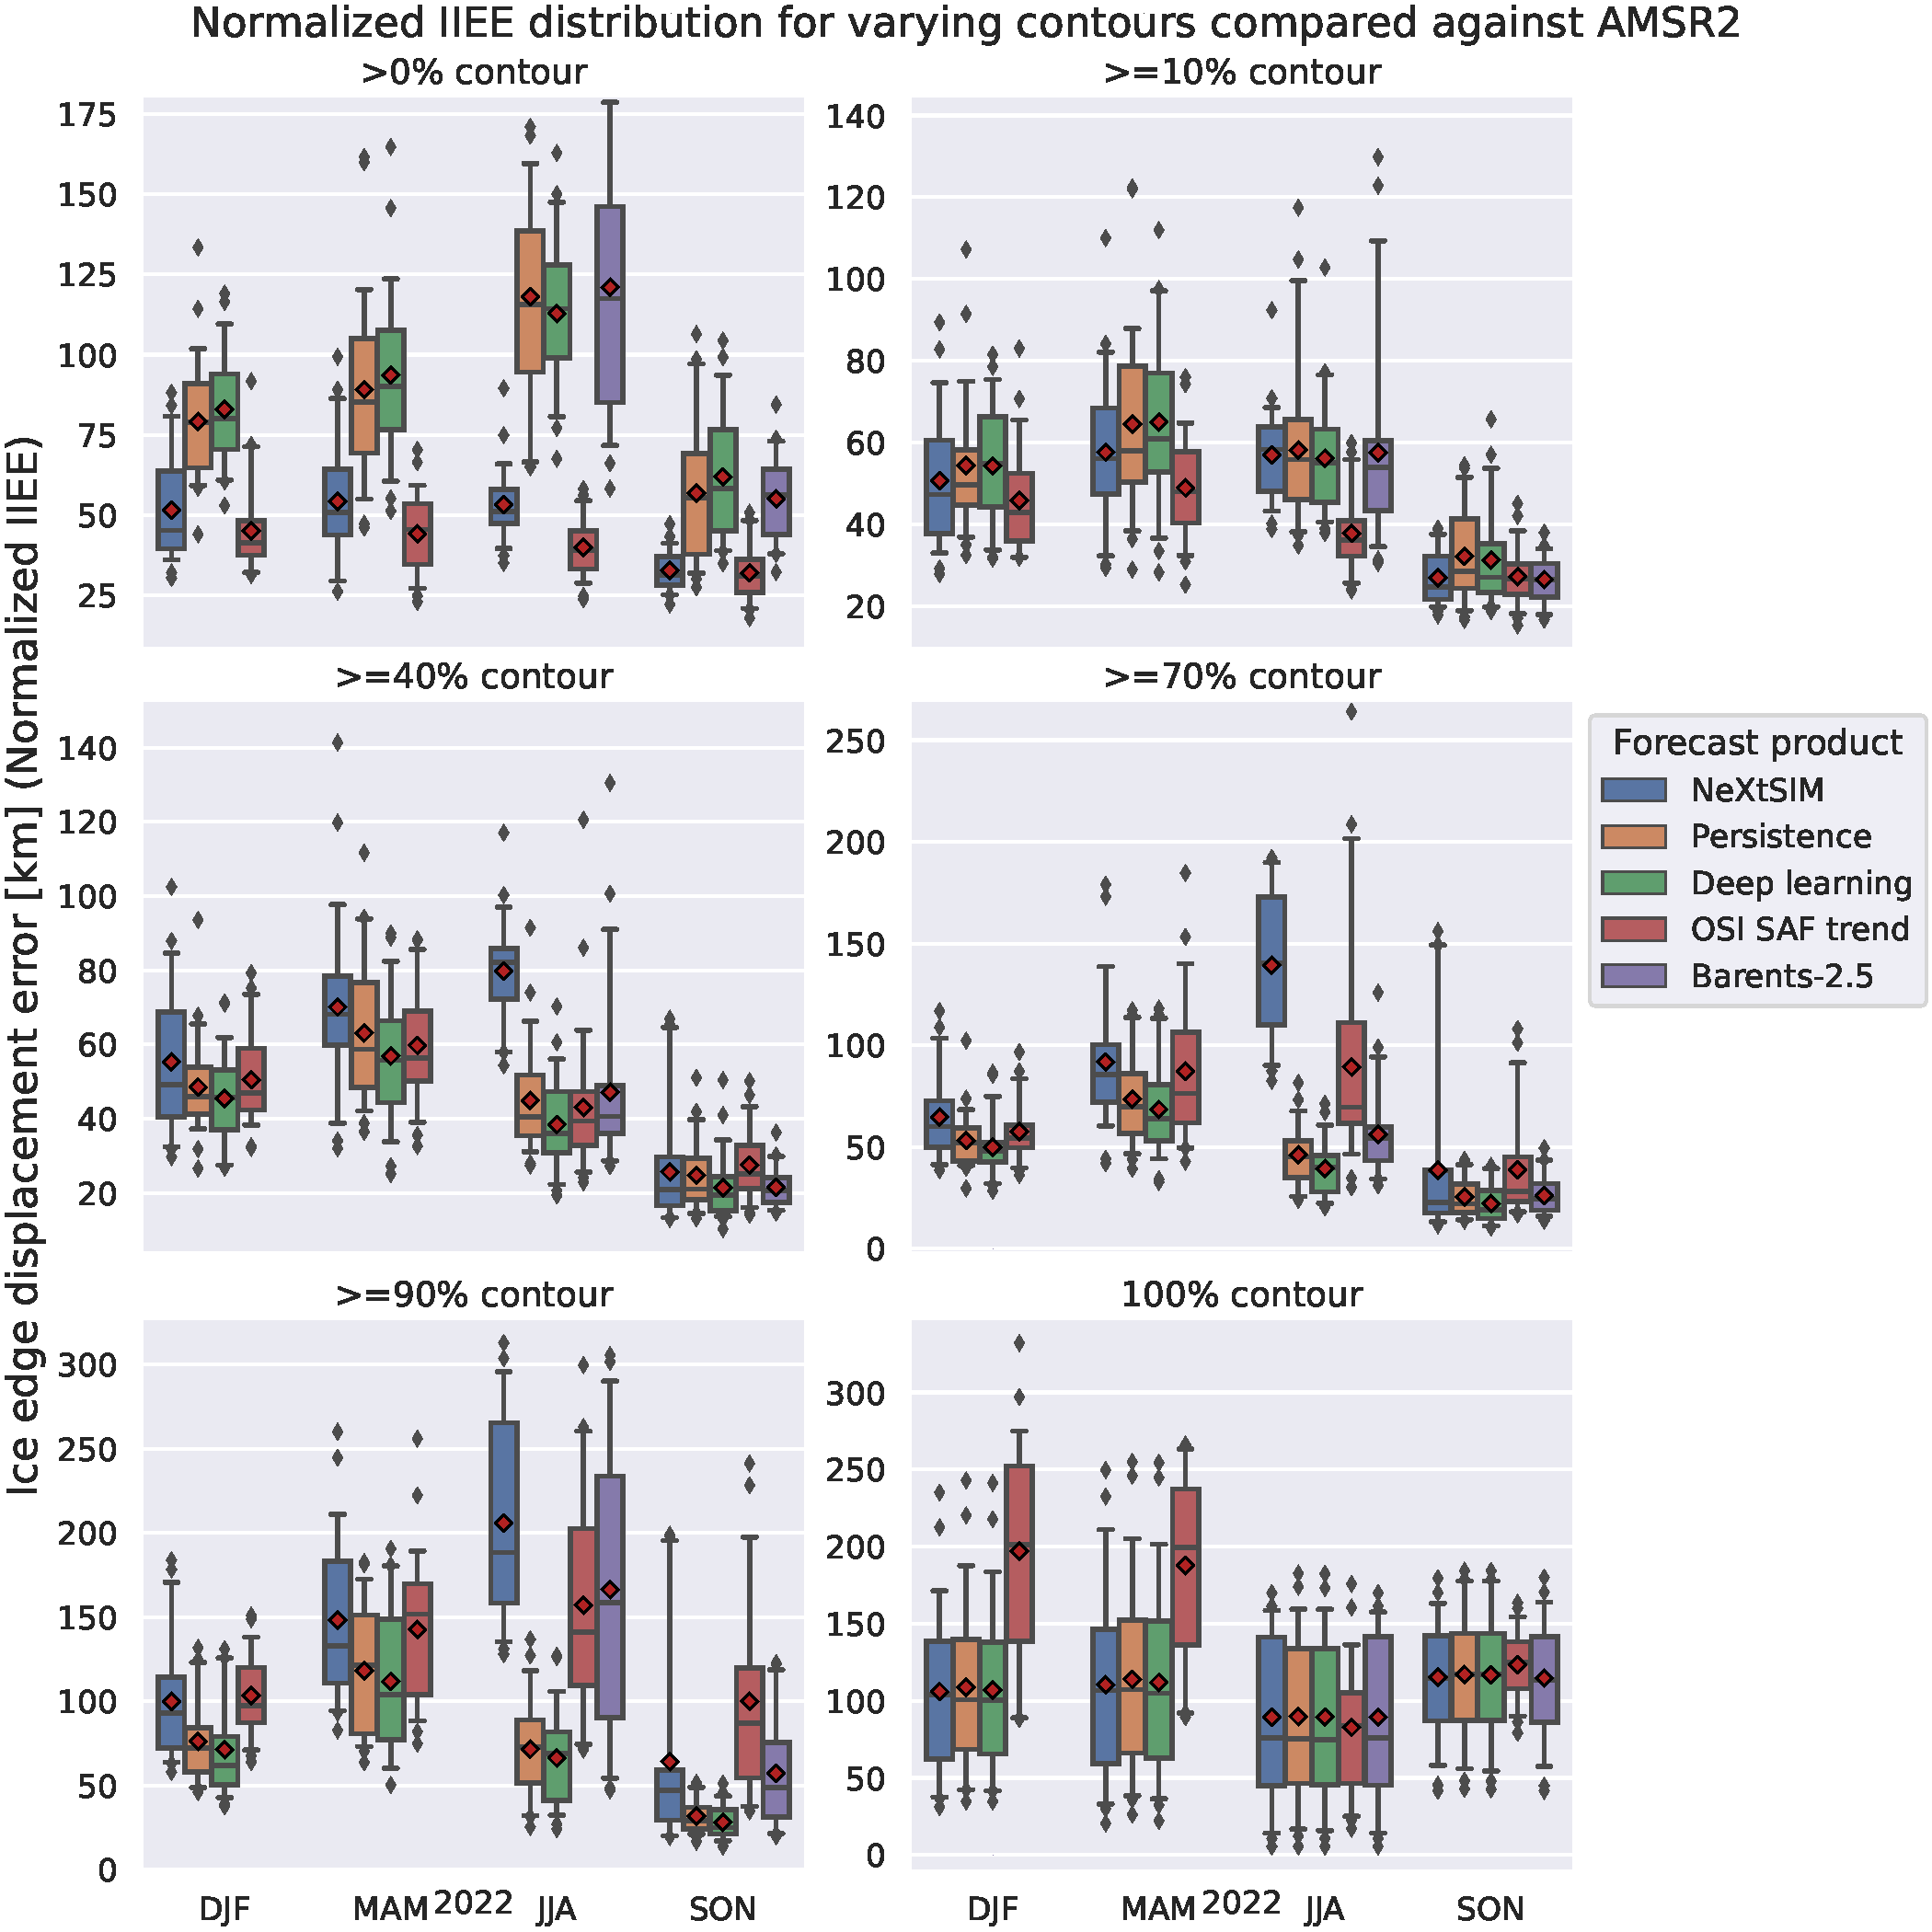
\includegraphics[width=\textwidth]{model_intercomparisson_amsr2.pdf}
    \caption{\label{fig:model_compare_amsr2}Same as Figure \ref{fig:model_compare}, but with AMSR2 sea ice concentration as the ground truth data. Note that AMSR2 is only used as reference for validation, not as target variable for training the deep learning system (Section \ref{sec:interproduct-compare})}
\end{figure}

Following the result seen in the upper leftmost distribution in Figure \ref{fig:model_compare_amsr2}, Figure \ref{fig:model_compare_amsr2_reduced} shows a comparable result but with a deep learning model which does not target the <10\% and fast-ice contours as described in Section \ref{sec:modifyhyperparam}. By inspecting the $<10\%$ contour, it can be seen that the deep learning system achieves significantly lower NIIEE than persistence, as well as the deep learning system in Figure \ref{fig:model_compare_amsr2}. Otherwise for the other contours, the performance of the deep learning system is comparable to the deep learning system in Figure \ref{fig:model_compare_amsr2}.

\begin{figure}
    \centering
    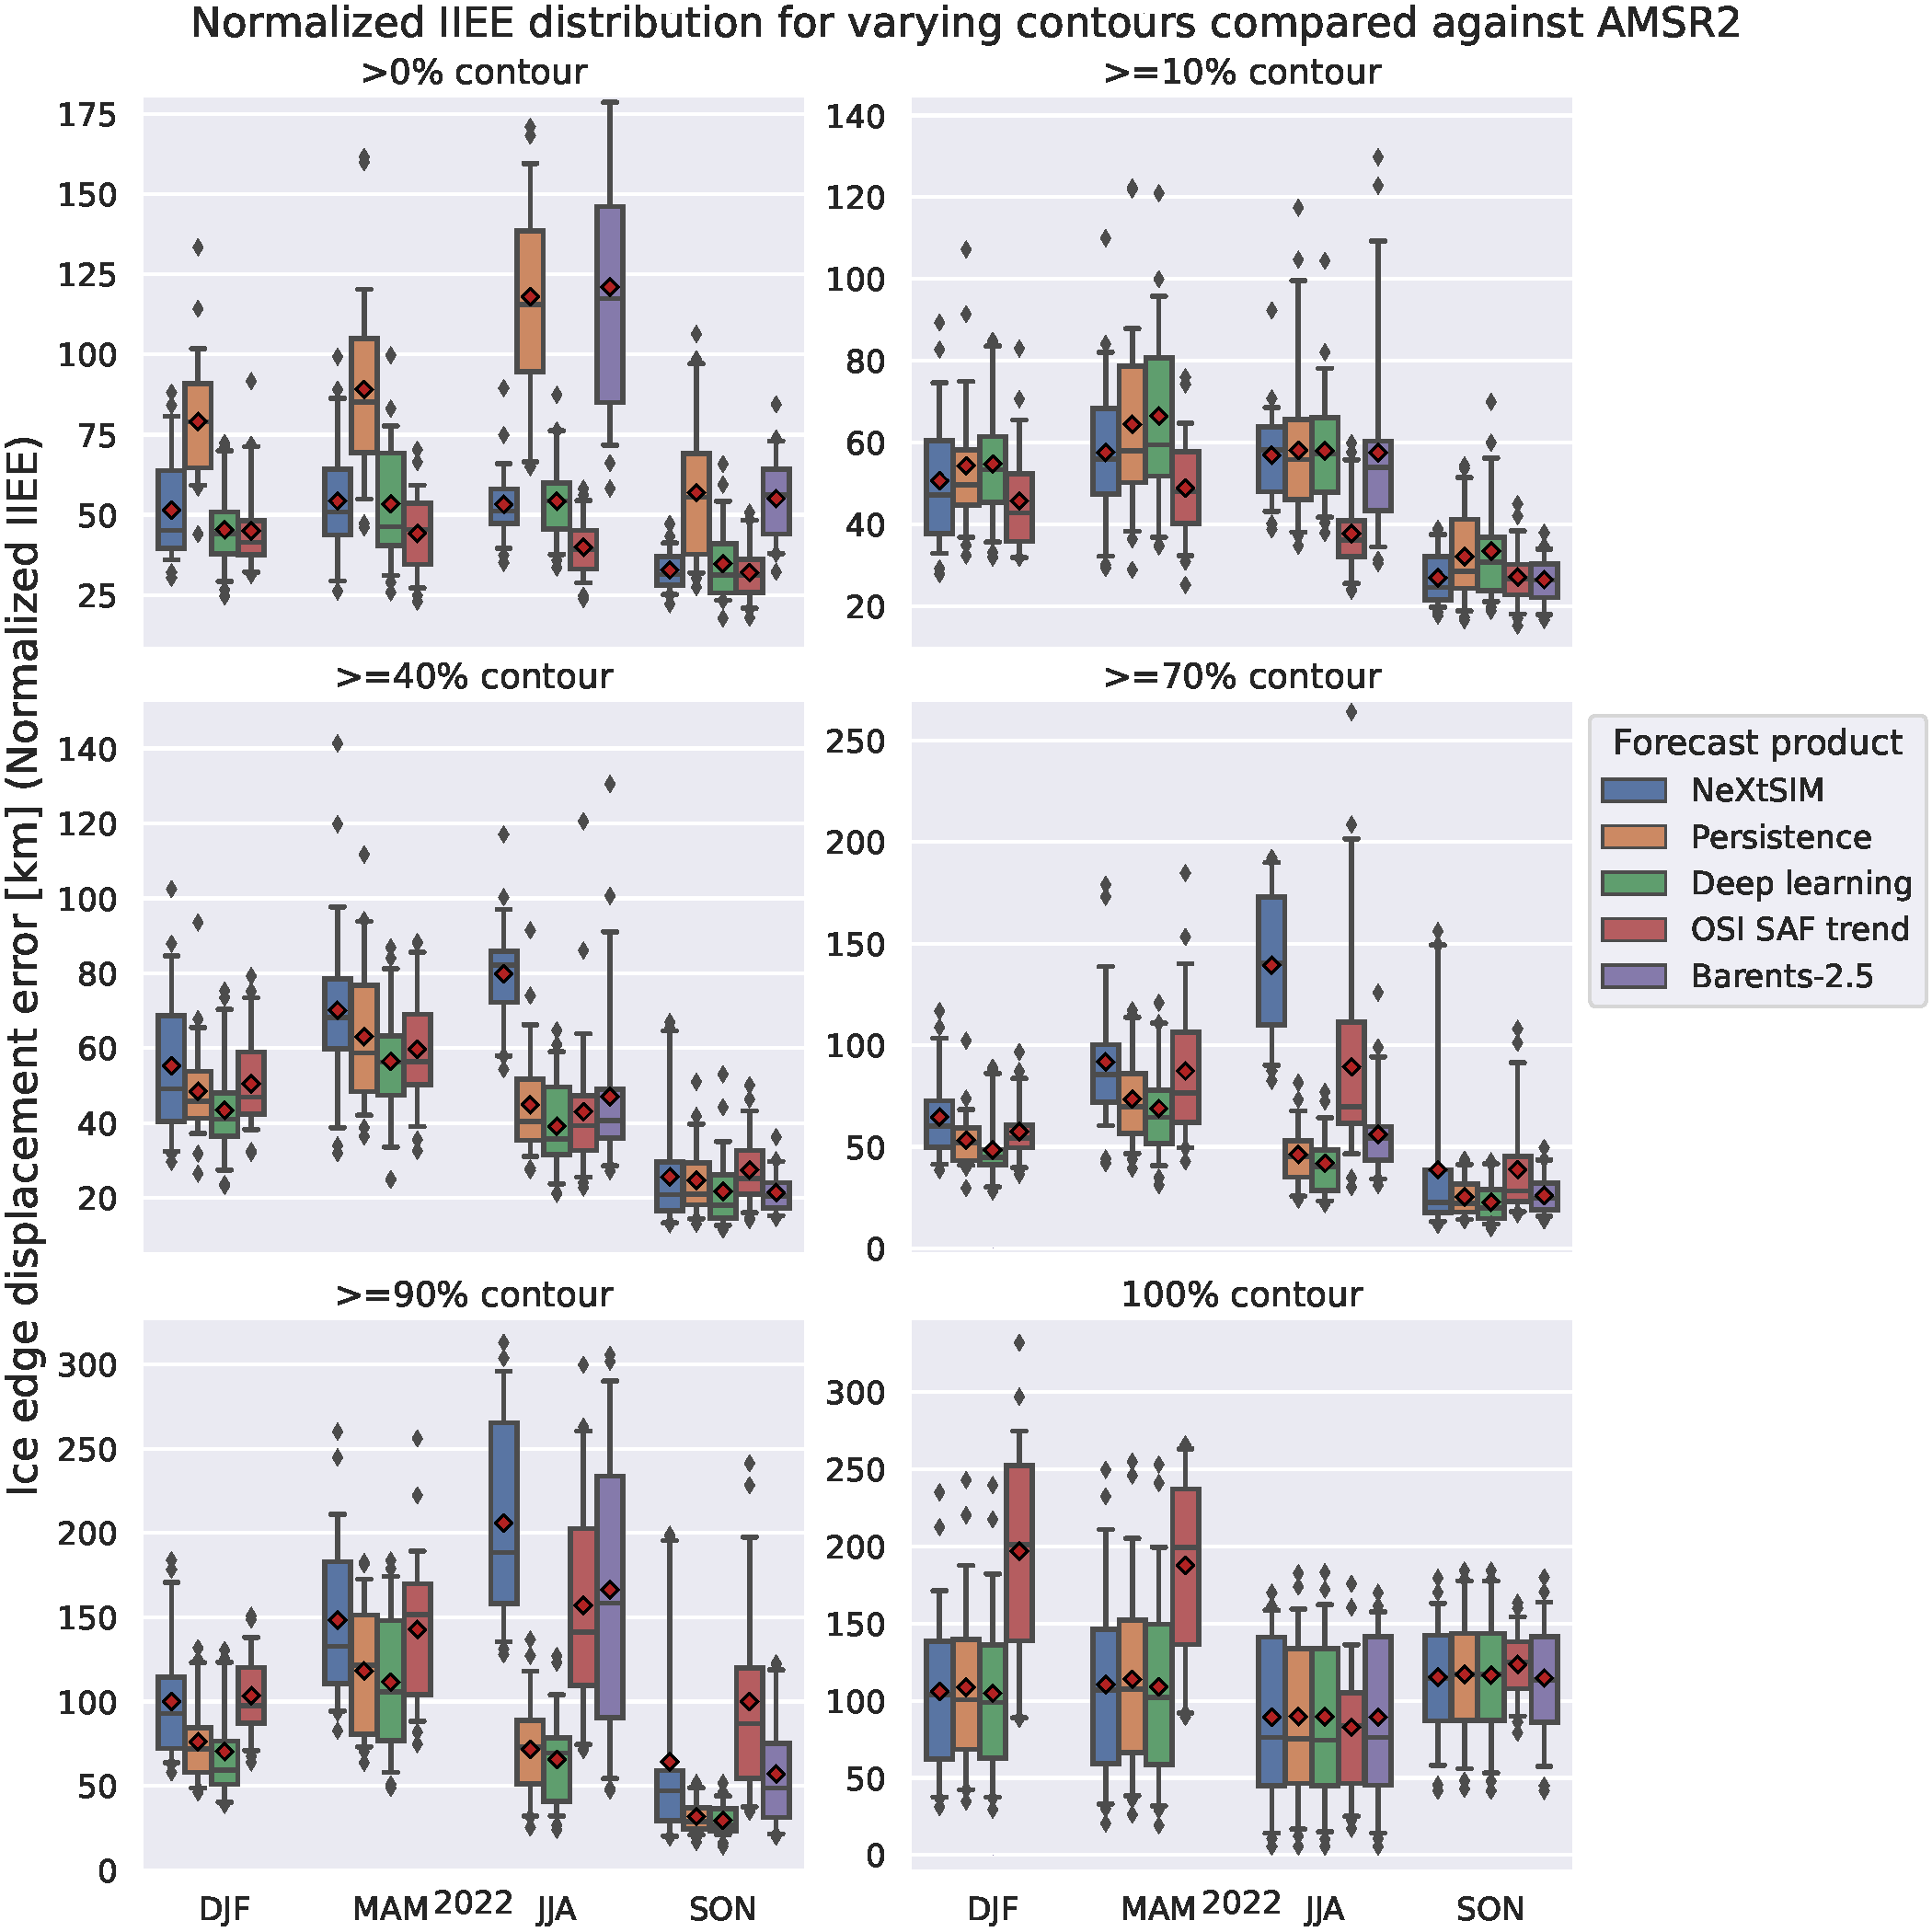
\includegraphics[width=\textwidth]{model_intercomparisson_amsr2_reduced.pdf}
    \caption{\label{fig:model_compare_amsr2_reduced}Same as Figure \ref{fig:model_compare_amsr2}, but the deep learning system used has reduced output classes.}
\end{figure}

\biblio
\end{document}